\documentclass[UTF8]{ctexart}
\CTEXsetup[format={\Large\bfseries}]{section}%一级标题居左
\usepackage{geometry}
\geometry{
	left=1.5cm, % 左边距,适用于装订
	right=2cm, % 右边距
	top=2.5cm, % 顶部边距
	bottom=2cm, % 底部边距
	bindingoffset=5mm % 装订偏移量,确保文本不会被装订覆盖
}
\usepackage{graphicx}
\usepackage{fancyhdr}
\usepackage[title]{appendix}
\usepackage{listings}
\usepackage{xcolor}
\usepackage{caption}
\usepackage{subcaption}

\lstset{
	basicstyle=\ttfamily\small,
	numbers=left,
	numberstyle=\scriptsize,
	numbersep=5pt,
	backgroundcolor=\color{white},
	showspaces=false,
	showstringspaces=false,
	showtabs=false,
	frame=single,
	tabsize=2,
	captionpos=t, % 将标题放在顶部
	breaklines=true,
	breakatwhitespace=false,
	escapeinside={\%*}{*)},
	extendedchars=false,
	linewidth=\linewidth,
	language=C
}
\pagestyle{fancy}	
\lhead{}
\chead{}
\rhead{\bfseries\textsl{物联网控制技术}}
\lfoot{}
\cfoot{\thepage}
\rfoot{}
\renewcommand{\headrulewidth}{0.6pt}    %单线页眉的设置 
\renewcommand{\footrulewidth}{0.4pt}     %单线页脚的设置 
%-----------双线页眉的设置  
\makeatletter 
\def\headrule{{\if@fancyplain\let\headrulewidth\plainheadrulewidth\fi%
		\hrule\@height 1.0pt \@width\headwidth\vskip1pt%上面线为1pt粗  
		\hrule\@height 0.5pt\@width\headwidth  %下面0.5pt粗            
		\vskip-2\headrulewidth\vskip-4pt}      %两条线的距离1pt        
		  \vspace{2mm}}     %双线与下面正文之间的垂直间距 
\makeatother    
%------------双线页眉的设置            
% \usepackage{booktabs}
 %\usepackage{subfigure}
\usepackage{setspace}
\usepackage{amsmath}
\usepackage{array}%需要该宏包
\usepackage{diagbox} % 加载宏包
\usepackage{multirow}
\usepackage{textcomp}
\usepackage{indentfirst}%首行缩进宏包
\usepackage{setspace}
\usepackage{amssymb}
\title{{\heiti  {\LARGE 模糊\textbf{PID}控制驱动的节能温控风扇 }}\vspace{-2em}}
\date{}
\setlength{\headsep}{28pt}
\begin{document}
\thispagestyle{empty}
\begin{figure}[tph!]
	\centering
	
\includegraphics[width=0.77\linewidth]{figure/3}
\end{figure}

\begin{center}
	\quad \\
	\quad \\
	\quad \\
	\quad \\
	\heiti \fontsize{32}{17} 物\;\,联\;\,网\;\,控\;\,制\;\,技\;\,术\;\,实\;\,验\;\,报\;\,告
	\vskip 0.5cm
	\songti \zihao{2} 模糊PID控制驱动的节能温控风扇
\end{center}
\vskip 1cm

\begin{quotation}
	\songti \fontsize{24}{24}
	\doublespacing
	\par\setlength\parindent{12em}
	\qquad
	\begin{center}
		{\Large \textbf{学\hspace{0.88cm} 院:}\underline{\hbox to 58mm{\;\;\,\,信息技术学院\,\,\;\;}}}
		\vskip 0.32cm	
		{\Large 班\hspace{0.88cm} 级:\underline{\hbox to 58mm{\,\,\,物联网工程二班\,\,\,}}}
		\vskip 0.32cm
		{\Large 姓\hspace{0.88cm} 名:\underline{\hbox to 58mm{\centering {\;\;\;\;\;\;\;\;\;\;\;\;\;\;\,\,张景\,\,\;\;\;\;\;\;\;\;\;\;\;\;\;\;}}}}
		\vskip 0.32cm	
		{\Large 学\hspace{0.88cm} 号:\underline{\hbox to 58mm{\centering{\;\;\qquad2\,2\,1\,2\,1\,0\,0\,4\,1\,6}}}}
		\vskip 0.32cm	
		{\Large 指导教师:\underline{\hbox to 58mm{\centering {\;\;\;\;\;\;\;\;\,\,\,\,\;王光耀\;\,\,\,\,\;\;\;\;\;\;\;\;}}}}
	\end{center}	
	\vskip 5cm
	\begin{flushright}
		\zihao{4}2025\;年\;6\;月\;6\;日
	\end{flushright}
\end{quotation}
\newpage
\thispagestyle{empty}
%\tableofcontents
\maketitle	
\thispagestyle{fancy}	
\section{实验目的}
本实验旨在设计并实现一个基于ESP32-C6平台的模糊PID温度控制系统,通过DHT11传感器采集环境温度数据,结合模糊控制策略动态调整PID参数,并使用PWM驱动风扇电机调节转速,从而实现对目标温度的快速响应和稳定控制。具体目标如下:
	\begin{enumerate}
		\item 掌握 ESP32 开发环境的搭建及 FreeRTOS 多任务编程;
		\item 学习使用 DHT11 温湿度传感器进行数据采集;
		\item 熟悉 OLED 屏幕的初始化与数据显示;
		\item 掌握模糊控制与PID控制相结合的算法实现;
		\item 实现闭环温度反馈控制,提升系统的鲁棒性与自适应能力;
		\item 综合应用硬件驱动、传感器采集、控制算法和人机交互,提升嵌入式系统开发能力。
	\end{enumerate}
\section{功能模块设计}
本系统基于 ESP32 嵌入式平台开发,结合 DHT11 温湿度传感器、OLED 显示屏和 L9110H 电机驱动模块,构建了一个具备环境感知、数据可视化与自动控制能力的模糊 PID 控制系统。整个系统以 FreeRTOS 实时操作系统为基础,采用多任务并发机制,实现对温湿度信息的采集、显示以及基于模糊逻辑的智能调节。
\subsection{主控模块}
本次系统设计的微处理芯片采用 FireBeetle 2 ESP32-C6 芯片,支持 2.4 GHz Wi-Fi 6、Bluetooth 5、Zigbee 3.0 及 Thread 1.3 的系统级芯片 (SoC),集成了高性能 RISC-V 32 位处理器和低功耗 RISC-V 32 位处理器、Wi-Fi、Bluetooth LE、802.15.4 基带和 MAC、RF 模块及外设等。

\begin{itemize}
	\item 硬件引脚接线:
	\begin{enumerate}
		\item DHT11 传感器:
		\begin{itemize}
			\item 数据引脚:连接到 GPIO1
			\item 电源引脚:连接到 3.3V
			\item 地引脚:连接到 GND
		\end{itemize}
		\item OLED显示屏:
		\begin{itemize}
			\item SCL 引脚:连接到 GPIO4
			\item SDA 引脚:连接到 GPIO3
			\item 电源引脚:连接到 3.3V
			\item 地引脚:连接到 GND
		\end{itemize}
		\item 电机驱动模块:
		\begin{itemize}
			\item INA 引脚:连接到 GPIO7(PWM 输出)。
			\item INB 引脚:连接到 GPIO6(方向控制)。
			\item 电源引脚:连接到外部电源。
			\item 地引脚:连接到 GND。
		\end{itemize}
	\end{enumerate}
	\begin{figure}[htbp]
		\centering
		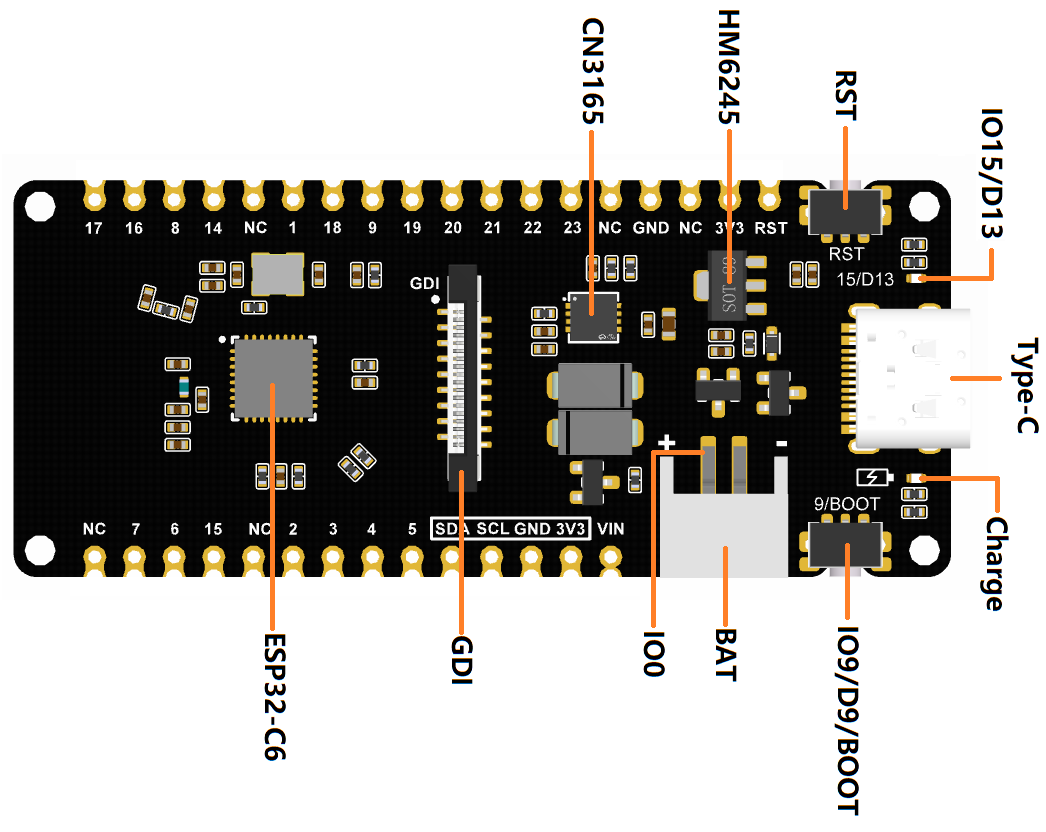
\includegraphics[width=0.42\linewidth]{figure/7}
		\caption{ESP32C6芯片} % 图片标题
		\label{fig:image1} % 图片标签,用于在文中引用
	\end{figure}
	\item 模块实现的功能
	\begin{enumerate}
		\item 数据采集:通过连接 DHT11 温湿度传感器,采集环境的温度和湿度数据。
		\item 数据处理:使用模糊控制算法,根据采集的温湿度数据计算控制输出,用于调节电机速度。
		\item 通信与显示:通过 I2C 接口与 OLED 显示屏通信,实时显示温湿度数据和控制输出。
		\item 任务调度:使用 FreeRTOS 实现多任务并行运行,包括传感器数据采集任务、模糊控制任务和电机控制任务。
	\end{enumerate}
\end{itemize}
\subsection{数据采集模块}
本模块基于 DHT11 温湿度传感器进行环境数据采集。DHT11 是一款数字温湿度传感器,通过单总线协议与主控芯片通信,具有较高的稳定性和较低的成本。
	\begin{figure}[htbp]
	\centering
	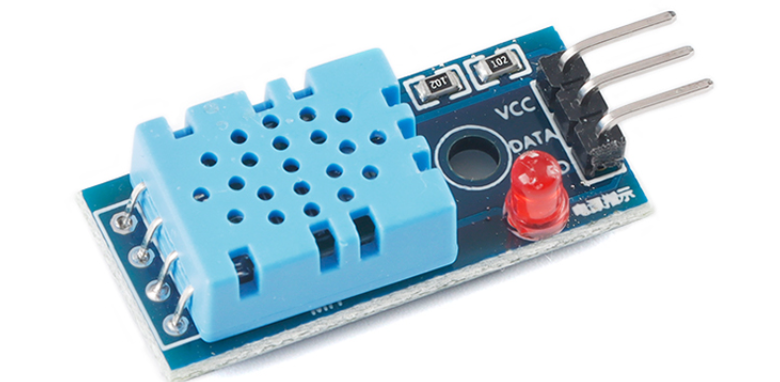
\includegraphics[width=0.3\linewidth]{figure/2}
	\caption{DHT11温湿度传感器} % 图片标题
	\label{fig:image1} % 图片标签,用于在文中引用
\end{figure}
\begin{itemize}
	\item 模块实现的	功能:
	\begin{enumerate}
		\item 实现对当前环境温度和湿度的周期性采集;
		\item 支持浮点数格式输出,提高精度;
		\item 通过 GPIO 引脚与 ESP32 进行双向通信;
		\item 提供错误检测机制,确保数据完整性。
	\end{enumerate}
	\item DHT11的工作原理:DHT11 通过单总线协议与主机通信,传输温度数据。
	
	\begin{enumerate}
		\item 初始化阶段
			\begin{itemize}
				\item 主机(MCU)通过拉低信号线向 DH11 发送启动信号。
				\item DHT11 接收到启动信号后,拉低信号线 80μs,然后拉高信号线 80μs,表示准备好发送数据。
			\end{itemize}
		\item 数据传输阶段
		\begin{itemize}
			\item DH11 通过单总线协议发送 40 位数据(5 字节),包括湿度和温度信息。
			\item 数据格式:前 8 位:湿度整数部分。中间 8 位:湿度小数部分。接着 8 位:温度整数部分。再接 8 位:温度小数部分。最后 8 位:校验和(前 4 字节的和)。
		\end{itemize}
		\item 数据位的编码\par
		
			 每一位数据通过高电平的持续时间来表示:
			\begin{itemize}
				\item 低电平 50μs + 高电平 26-28μs:表示逻辑 0。
				\item 低电平 50μs + 高电平 70μs:表示逻辑 1。
			\end{itemize}

		\item 校验阶段
		\begin{itemize}
			\item 主机接收完 40 位数据后,计算前 4 字节的和,与校验和进行比较。
			\item 如果校验通过,则数据有效;否则数据无效。
		\end{itemize}
	\end{enumerate}
	\begin{figure}[htbp]
		\centering
		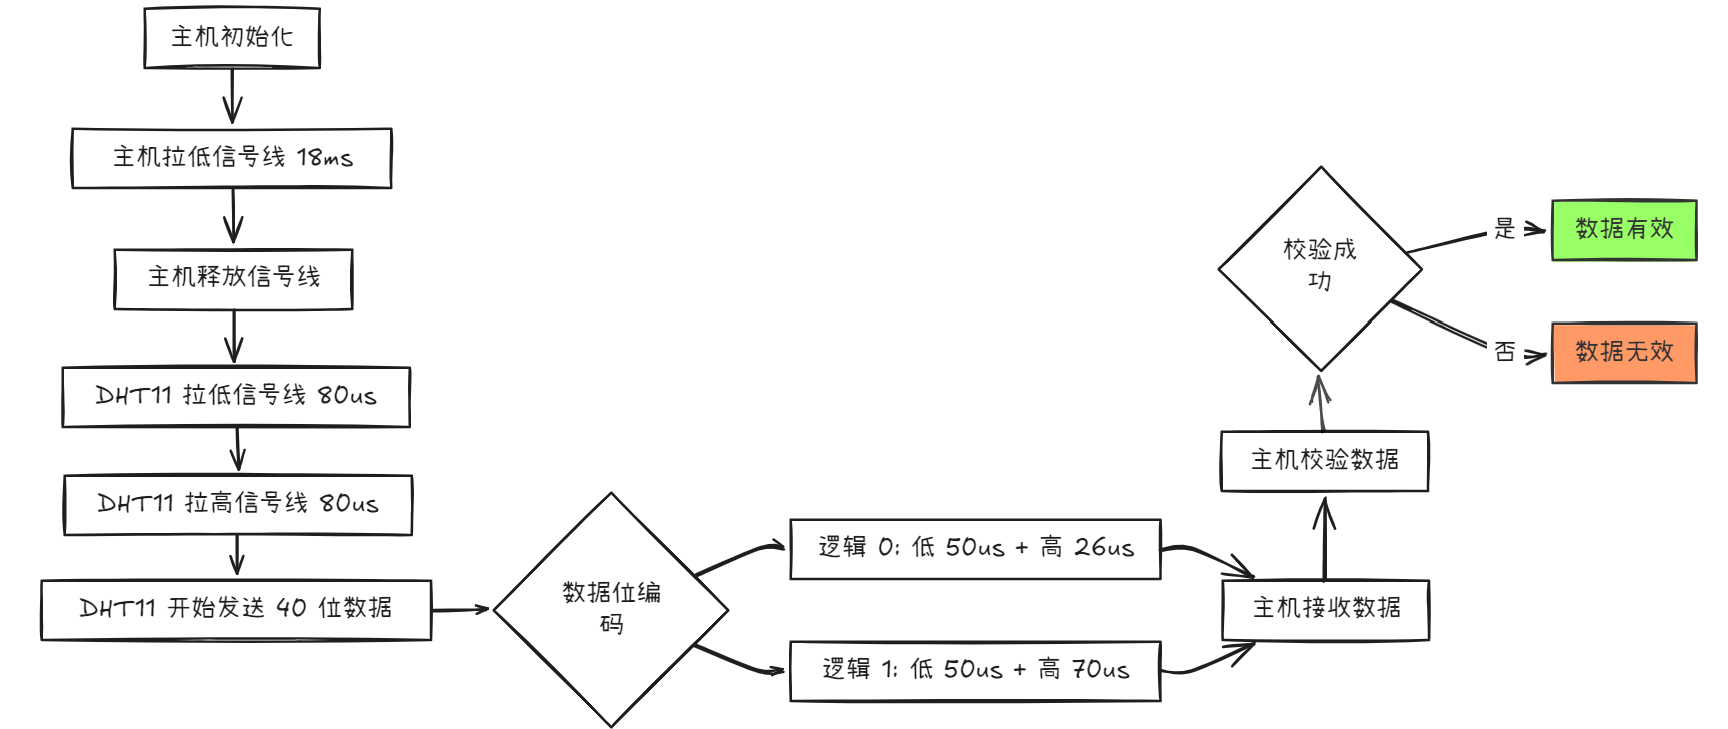
\includegraphics[width=0.98\linewidth]{figure/4}
		\caption{DHT11工作流程图} % 图片标题
		\label{fig:image2} % 图片标签,用于在文中引用
	\end{figure}
	
\end{itemize}
\subsection{显示模块}
关于显示模块,本次实验我采用了 ssd1306 模块,它是一种自发光显示技术,利用有机材料在电流作用下发光。它具有高对比度、低功耗、广视角等优点。
\begin{figure}[htbp]
	\centering
	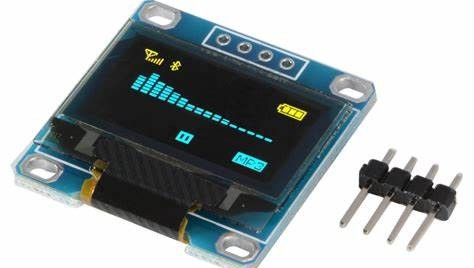
\includegraphics[width=0.28\linewidth]{figure/5}
	\caption{ssd1306显示屏} % 图片标题
	\label{fig:image3} % 图片标签,用于在文中引用
\end{figure}
\begin{itemize}
	\item 模块实现的功能:对系统检测到的温湿度进行实时显示,并当 DHT11 传感器读取失败时,提示错误信息。
	\item ssd1306 的工作原理:
	\begin{itemize}
		\item 像素发光:OLED显示屏由多个像素组成,每个像素包含红、绿、蓝(RGB)子像素。当电流通过有机材料时,材料发光,形成图像。
		\item 驱动方式:OLED 显示屏通常采用矩阵驱动方式,通过行列扫描控制像素点亮。
		\item 通信协议:OLED 显示屏通常通过 I2C 或 SPI 接口与主机通信。主机通过发送命令和数据控制 OLED 的显示内容。
		\item 显示内容更新:显存数组存储当前显示内容。更新显示时,显存数据通过通信接口发送到 OLED 显示屏。
	\end{itemize}
\end{itemize}
\begin{figure}[htbp]
	\centering
	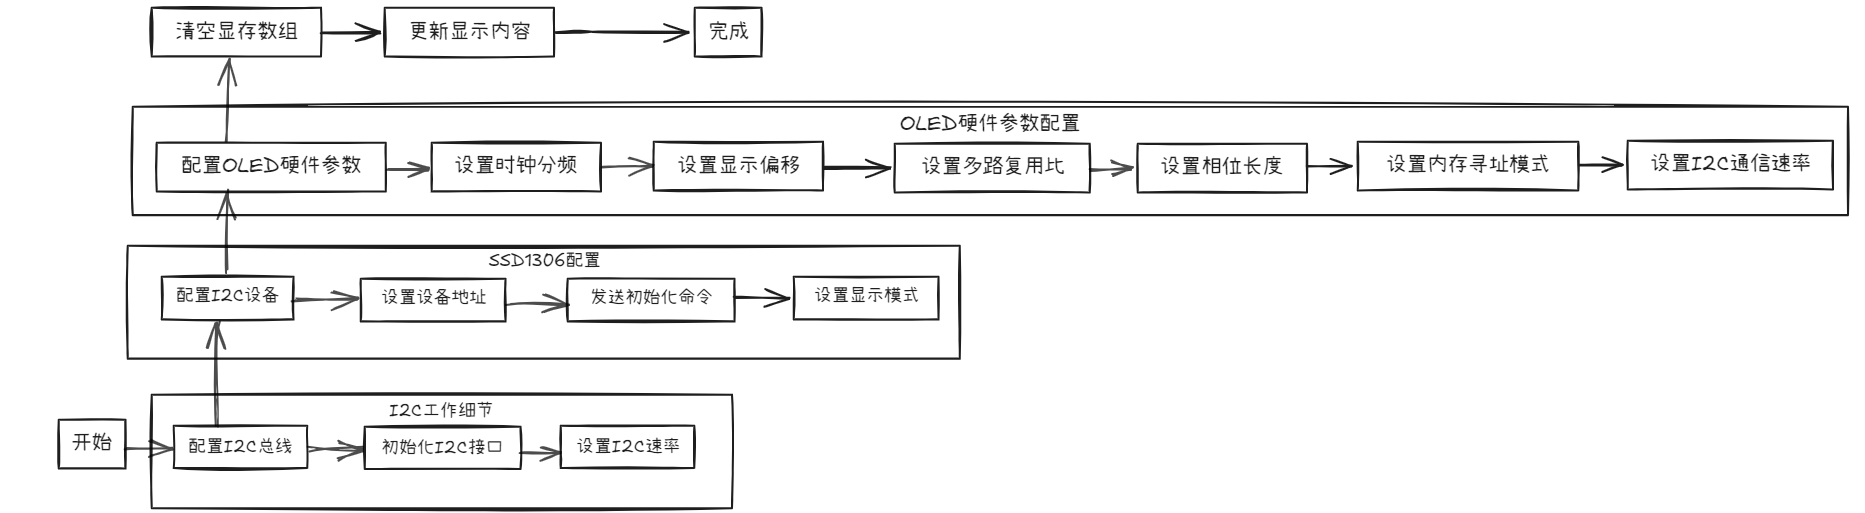
\includegraphics[width=1\linewidth]{figure/6}
	\caption{ssd1306显示工作原理} % 图片标题
	\label{fig:image4} % 图片标签,用于在文中引用
\end{figure}

\subsection{电机控制模块}
本次实验采用L9110H作为被控对象,它是一种双通道推挽式功率放大器集成电路,广泛应用于电机驱动、继电器控制以及小型电磁阀驱动等场景。它能够提供较高的输出电流,并且具备良好的热稳定性和可靠性。该芯片内部集成了两个NPN和PNP晶体管对,可以实现对负载的正向和反向驱动控制。
\begin{figure}[htbp]
	\centering
	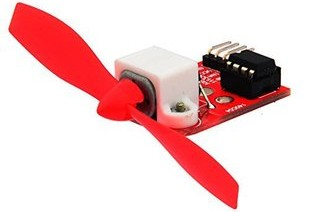
\includegraphics[width=0.21\linewidth]{figure/8}
	\caption{L9110H电机模块} % 图片标题
	\label{fig:image5} % 图片标签,用于在文中引用
\end{figure}\par
\begin{itemize}
	\item 模块实现的功能:
	\begin{itemize}
		\item PWM输出:通过 PWM 信号控制电机的速度。
		\item 方向控制:通过 GPIO 引脚连接INA与INB,控制电机的转速和旋转方向。
		\item 实时调节:根据模糊控制器的输出实时调整电机速度。
	\end{itemize}
	\item L9110H电机工作原理:
	\begin{itemize}
		\item 初始化:配置 GPIO 引脚,连接电机驱动模块的INA、INB。
		\item 速度控制:根据模糊控制器的输出设置 PWM 占空比。
		\item 方向控制:通过控制电机两端的电压来实现对电机旋转方向的控制。
	\end{itemize}
\end{itemize}
\subsection{模糊 PID 控制模块}
控制算法模块是整个系统的核心部分,采用模糊PID控制策略,结合模糊逻辑与经典PID控制的优势,实现对风扇转速的智能调节。系统首先通过DHT11传感器获取当前温度,计算温度误差及其变化率,并利用三角隶属度函数将输入变量模糊化为低、中、高三档;随后根据预设的模糊规则库进行加权推理,得出PID参数的增量值;接着动态更新PID控制器的Kp、Ki、Kd参数,使其适应当前系统状态;最后调用PID计算接口得到精确控制输出,并映射为PWM信号驱动风扇电机转动。整个过程在FreeRTOS任务中循环执行,形成闭环温控系统,提升了系统的响应速度与稳定性,同时具备良好的自适应能力。具体的流程如下 \ref{fig:mermaid} 所示:
\begin{figure}[htbp]
	\centering
	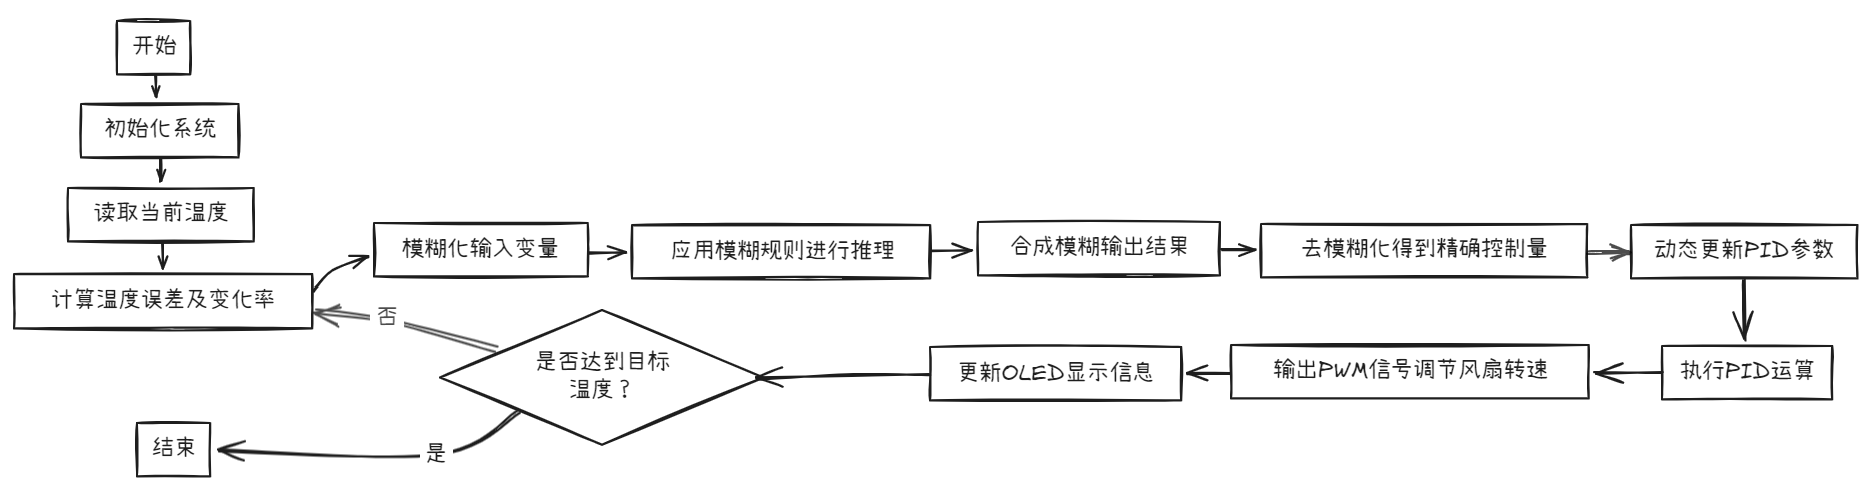
\includegraphics[width=1\linewidth]{figure/mermaid}
	\caption{模糊PID控制流程图}
	\label{fig:mermaid}
\end{figure}
\par 
\begin{itemize}
	\item 模糊控制模块:
	\begin{enumerate}
		\item 定义输入变量:温度误差(Error)及其变化率(Delta Error);
		\item 使用三角隶属函数将误差划分为三个模糊集合:low, medium, high;
		\item 建立模糊规则库,根据误差和变化率推理出对应的控制量;
		\item 采用重心法(Centroid Method)进行去模糊化处理,得到精确的控制输出。
	\end{enumerate}
	\item PID 控制模块:
	\begin{enumerate}
		\item 使用 ESP-IDF 提供的 PID 控制组件 pid\_ctrl.h 实现PID计算;
		\item 根据模糊推理结果动态更新PID参数(Kp, Ki, Kd);
		\item 选择位置型PID控制方式,输出范围限制在 [0, 255],适配PWM输出。
	\end{enumerate}
\end{itemize}
\section{软件设计}
软件设计部分基于ESP-IDF平台和FreeRTOS操作系统,采用模块化设计思想实现了模糊PID温控风扇系统的各项功能。主程序在app\_main函数中完成系统初始化后创建了一个核心任务fuzzy\_pid\_task,该任务周期性地读取DHT11传感器的温度数据,计算误差及其变化率,并通过模糊控制模块对输入变量进行模糊化处理;随后依据预设的模糊规则库进行加权推理,生成用于调整PID控制器的增量参数(ΔKp、ΔKi、ΔKd);更新后的参数被用于PID计算,得到精确的控制输出量,并映射为PWM信号驱动风扇电机运转;同时,OLED显示任务实时更新当前温度、湿度、误差及控制输出值,形成完整的闭环控制系统。整个软件架构充分利用了FreeRTOS的任务调度机制,确保了系统响应的实时性和控制的稳定性。
\begin{enumerate}
	\item 初始化与主循环逻辑:
	在main.c中完成了OLED显示屏、DHT温湿度传感器以及PWM电机驱动的初始化,并创建了一个FreeRTOS任务用于周期性执行模糊PID控制
	\begin{lstlisting}
		void fuzzy_pid_task(void *pvParameters)
		{
			while (1) {
				float temperature = read_temperature(); // 读取当前温度
				float error = target_temp - temperature; // 计算误差
				float delta_error = error - last_error; // 计算变化率
				FuzzyMembership error_memb = fuzzify_error(error);
				FuzzyMembership delta_error_memb = fuzzify_delta_error(delta_error);
				infer_pid(error_memb, delta_error_memb, &delta_kp, &delta_ki, &delta_kd);
				pid_update_parameters(pid, &new_params); // 更新PID参数
				pid_compute(pid, error, &control_output); // 执行PID计算
				set_motor_speed((int)control_output); // 输出PWM信号
				vTaskDelay(pdMS_TO_TICKS(1000)); // 延时1秒
			}
		}
	\end{lstlisting}
	\item 模糊控制算法实现:
	\begin{enumerate}
		\item 隶属度函数定义:采用三角隶属度函数对误差进行模糊化处理
		\begin{lstlisting}
			float triangle(float x, float a, float b, float c)
			{
				if (x <= a || x >= c) return 0.0;
				else if (x > a && x <= b) return (x - a) / (b - a);
				else return (c - x) / (c - b);
			}
			
			// 模糊化误差
			FuzzyMembership fuzzify_error(float error)
			{
				FuzzyMembership membership = {0.0, 0.0, 0.0};
				float e = (error < 0) ? 0 : error; // 负数直接归零
				membership.low = triangle(e, 0.0, 0.0, 10.0);
				membership.medium = triangle(e, 5.0, 10.0, 15.0);
				membership.high = triangle(e, 10.0, 20.0, 20.0);
				return membership;
			}
			// 模糊化误差变化
			FuzzyMembership fuzzify_delta_error(float delta_error)
			{
				FuzzyMembership membership = {0.0, 0.0, 0.0};
				float de = (delta_error < 0) ? 0 : delta_error; // 负数直接归零
				membership.high = triangle(de, 2.5, 5.0, 5.0);
				membership.medium = triangle(de, 1.25, 2.5, 3.75);
				membership.low = triangle(de, 0.0, 0.0, 2.5);
				return membership;
			}
		\end{lstlisting}
		\item 模糊规则推理:根据预设的模糊规则矩阵进行加权平均计算,得到PID参数增量
		\begin{lstlisting}
			static const float kp_rules[3][3] = {
				// ec: SMALL, MEDIUM, LARGE
				{0.2f, 1.0f, 1.8f}, // e: SMALL
				{2.0f, 2.5f, 3.0f}, // e: MEDIUM
				{3.0f, 4.0f, 6.0f}  // e: LARGE
			};
			static const float ki_rules[3][3] = {
				{0.03f, 0.08f, 0.14f},
				{0.08f, 0.12f, 0.18f},
				{0.14f, 0.18f, 0.2f}};
			static const float kd_rules[3][3] = {
				{0.0f, 0.5f, 0.7f},
				{0.5f, 0.8f, 1.0f},
				{0.7f, 1.0f, 1.2f}};
			void infer_pid(FuzzyMembership error_membership, 
			FuzzyMembership delta_error_membership, 
			float *delta_kp, float *delta_ki, float *delta_kd);
		\end{lstlisting}
		\item 模糊推理以及去模糊化处理:
		\begin{lstlisting}
			void infer_pid(FuzzyMembership error_membership, 
			FuzzyMembership delta_error_membership, float *delta_kp, float *delta_ki, float *delta_kd)
			{
				float kp = 0.0f, ki = 0.0f, kd = 0.0f; // 初始值设为0
				float total_weight = 0.0f;
				
				float e_memberships[3] = {error_membership.low, error_membership.medium, error_membership.high};
				float ec_memberships[3] = {delta_error_membership.low, delta_error_membership.medium, delta_error_membership.high};
				
				for (int e = 0; e < 3; e++)
					for (int ec = 0; ec < 3; ec++)
					{
						float weight = e_memberships[e] * ec_memberships[ec];
						kp += weight * kp_rules[e][ec];
						ki += weight * ki_rules[e][ec];
						kd += weight * kd_rules[e][ec];
						total_weight += weight;
					}
				
				// 解模糊化(加权平均)
				*delta_kp = (total_weight > 0) ? kp / total_weight : 0.0f;
				*delta_ki = (total_weight > 0) ? ki / total_weight : 0.0f;
				*delta_kd = (total_weight > 0) ? kd / total_weight : 0.0f;
			}
		\end{lstlisting}
		\item 本次设计的误差和误差率的隶属度函数如下:
		\begin{figure}[htbp]
			\centering
			\begin{subfigure}[b]{0.48\textwidth}
				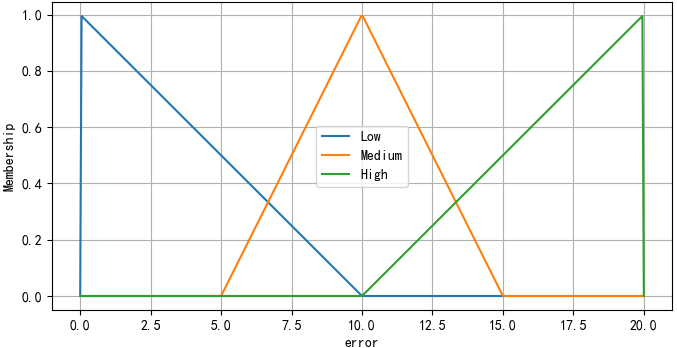
\includegraphics[width=\textwidth]{figure/f_e}
				\caption{fuzzify\_Error隶属度函数}
				\label{fig:subfig1}
			\end{subfigure}
			\hfill % 添加一些水平空间
			\begin{subfigure}[b]{0.47\textwidth}
				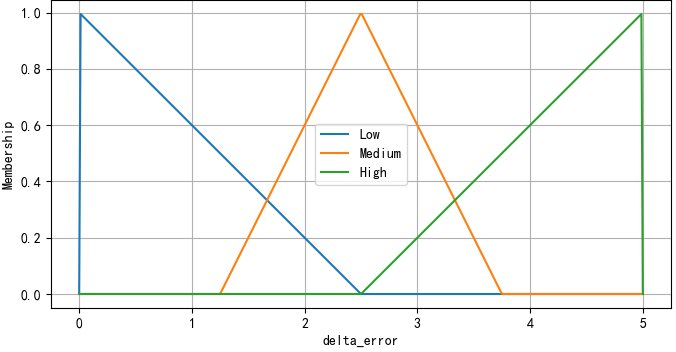
\includegraphics[width=\textwidth]{figure/Fd_e}
				\caption{fuzzify\_delta\_Error隶属度函数}
				\label{fig:subfig2}
			\end{subfigure}
			\caption{误差和误差率的隶属度函数}
			\label{fig:main}
		\end{figure}
	\end{enumerate}
	\item PID控制算法实现:
	\begin{enumerate}
		\item PID控制器初始化:创建PID控制块并设置初始参数
		\begin{lstlisting}
			pid_ctrl_config_t pid_config = {
				.init_param = {
					.kp = 10.8,
					.ki = 0.1,
					.kd = 0.06,
					.max_output = 255.0,
					.min_output = 0.0,
					.cal_type = PID_CAL_TYPE_POSITIONAL
				}
			};
		\end{lstlisting}
		\item 动态更新PID参数:根据模糊推理结果更新PID控制器的Kp/Ki/Kd参数
		\begin{lstlisting}
			float delta_kp,delta_ki,delta_kd;
			infer_pid(error_memb,delta_error_memb,&delta_kp,&delta_ki,&delta_kd);
			
			// 更新PID参数
			pid_ctrl_parameter_t new_params;
			new_params.kp = pid_config.init_param.kp + delta_kp;
			new_params.ki = pid_config.init_param.ki + delta_ki;
			new_params.kd = pid_config.init_param.kd + delta_kd;
			new_params.max_output = pid_config.init_param.max_output;
			new_params.min_output = pid_config.init_param.min_output;
			new_params.max_integral = pid_config.init_param.max_integral;
			new_params.min_integral = pid_config.init_param.min_integral;
			new_params.cal_type = pid_config.init_param.cal_type;
			pid_update_parameters(pid, &new_params);
		\end{lstlisting}
	\end{enumerate}
	\item PWM输出控制:计算出输出,并使用LEDC模块生成PWM信号驱动风扇电机:
	\begin{lstlisting}
		float control_output;
		if (pid_compute(pid, error, &control_output) == ESP_OK)
		{
			if (control_output > 255.0) control_output = 255.0;
			display_temp_hum(current_temp, hum, control_output);
			ESP_LOGI(TAG1, "Temp: %.2f, Hum: %.2f, Error: %.2f, Control Output: %.2f", current_temp, hum, error, control_output);
			if(delta_error != 0)
			set_motor_speed(control_output);
		}
		else ESP_LOGE(TAG1, "PID computation failed");
		last_error = error;
		void set_motor_speed(uint8_t speed)
		{
			if(speed > 255) speed = 255;
			ledc_set_duty(LEDC_LOW_SPEED_MODE, PWM_CHANNEL, speed);
			ledc_update_duty(LEDC_LOW_SPEED_MODE, PWM_CHANNEL);
		}
		
	\end{lstlisting}
\end{enumerate}\par
本实验的软件设计充分体现了嵌入式系统中模块化编程的思想,利用FreeRTOS多任务机制实现了高实时性的闭环控制。通过将模糊控制与经典PID控制相结合,系统具备了良好的自适应能力,在面对非线性、时变性强的温控场景时仍能保持稳定的控制效果。未来可进一步优化模糊规则库、引入增量型PID控制方式,并增加历史数据记录功能以辅助调试与调参。
\section{系统测试}
	验证系统各模块的功能是否正常,包括温湿度数据采集、模糊 PID 控制输出计算、电机速度调节以及 OLED 显示功能。
	\begin{itemize}
		\item 硬件环境:
		\begin{enumerate}
			\item 主控芯片:ESP32-C6
			\item 温湿度传感器:DHT11
			\item 电机驱动模块:L9110H
			\item 显示模块:OLED
		\end{enumerate}
		\item 软件环境:		
		\begin{enumerate}
			\item 开发工具:Visual Studio Code
			\item 编程语言:C
			\item FreeRTOS 任务调度系统
		\end{enumerate}
		\item 硬件接线,如下图所示:
		\begin{figure}[htbp]
			\centering
			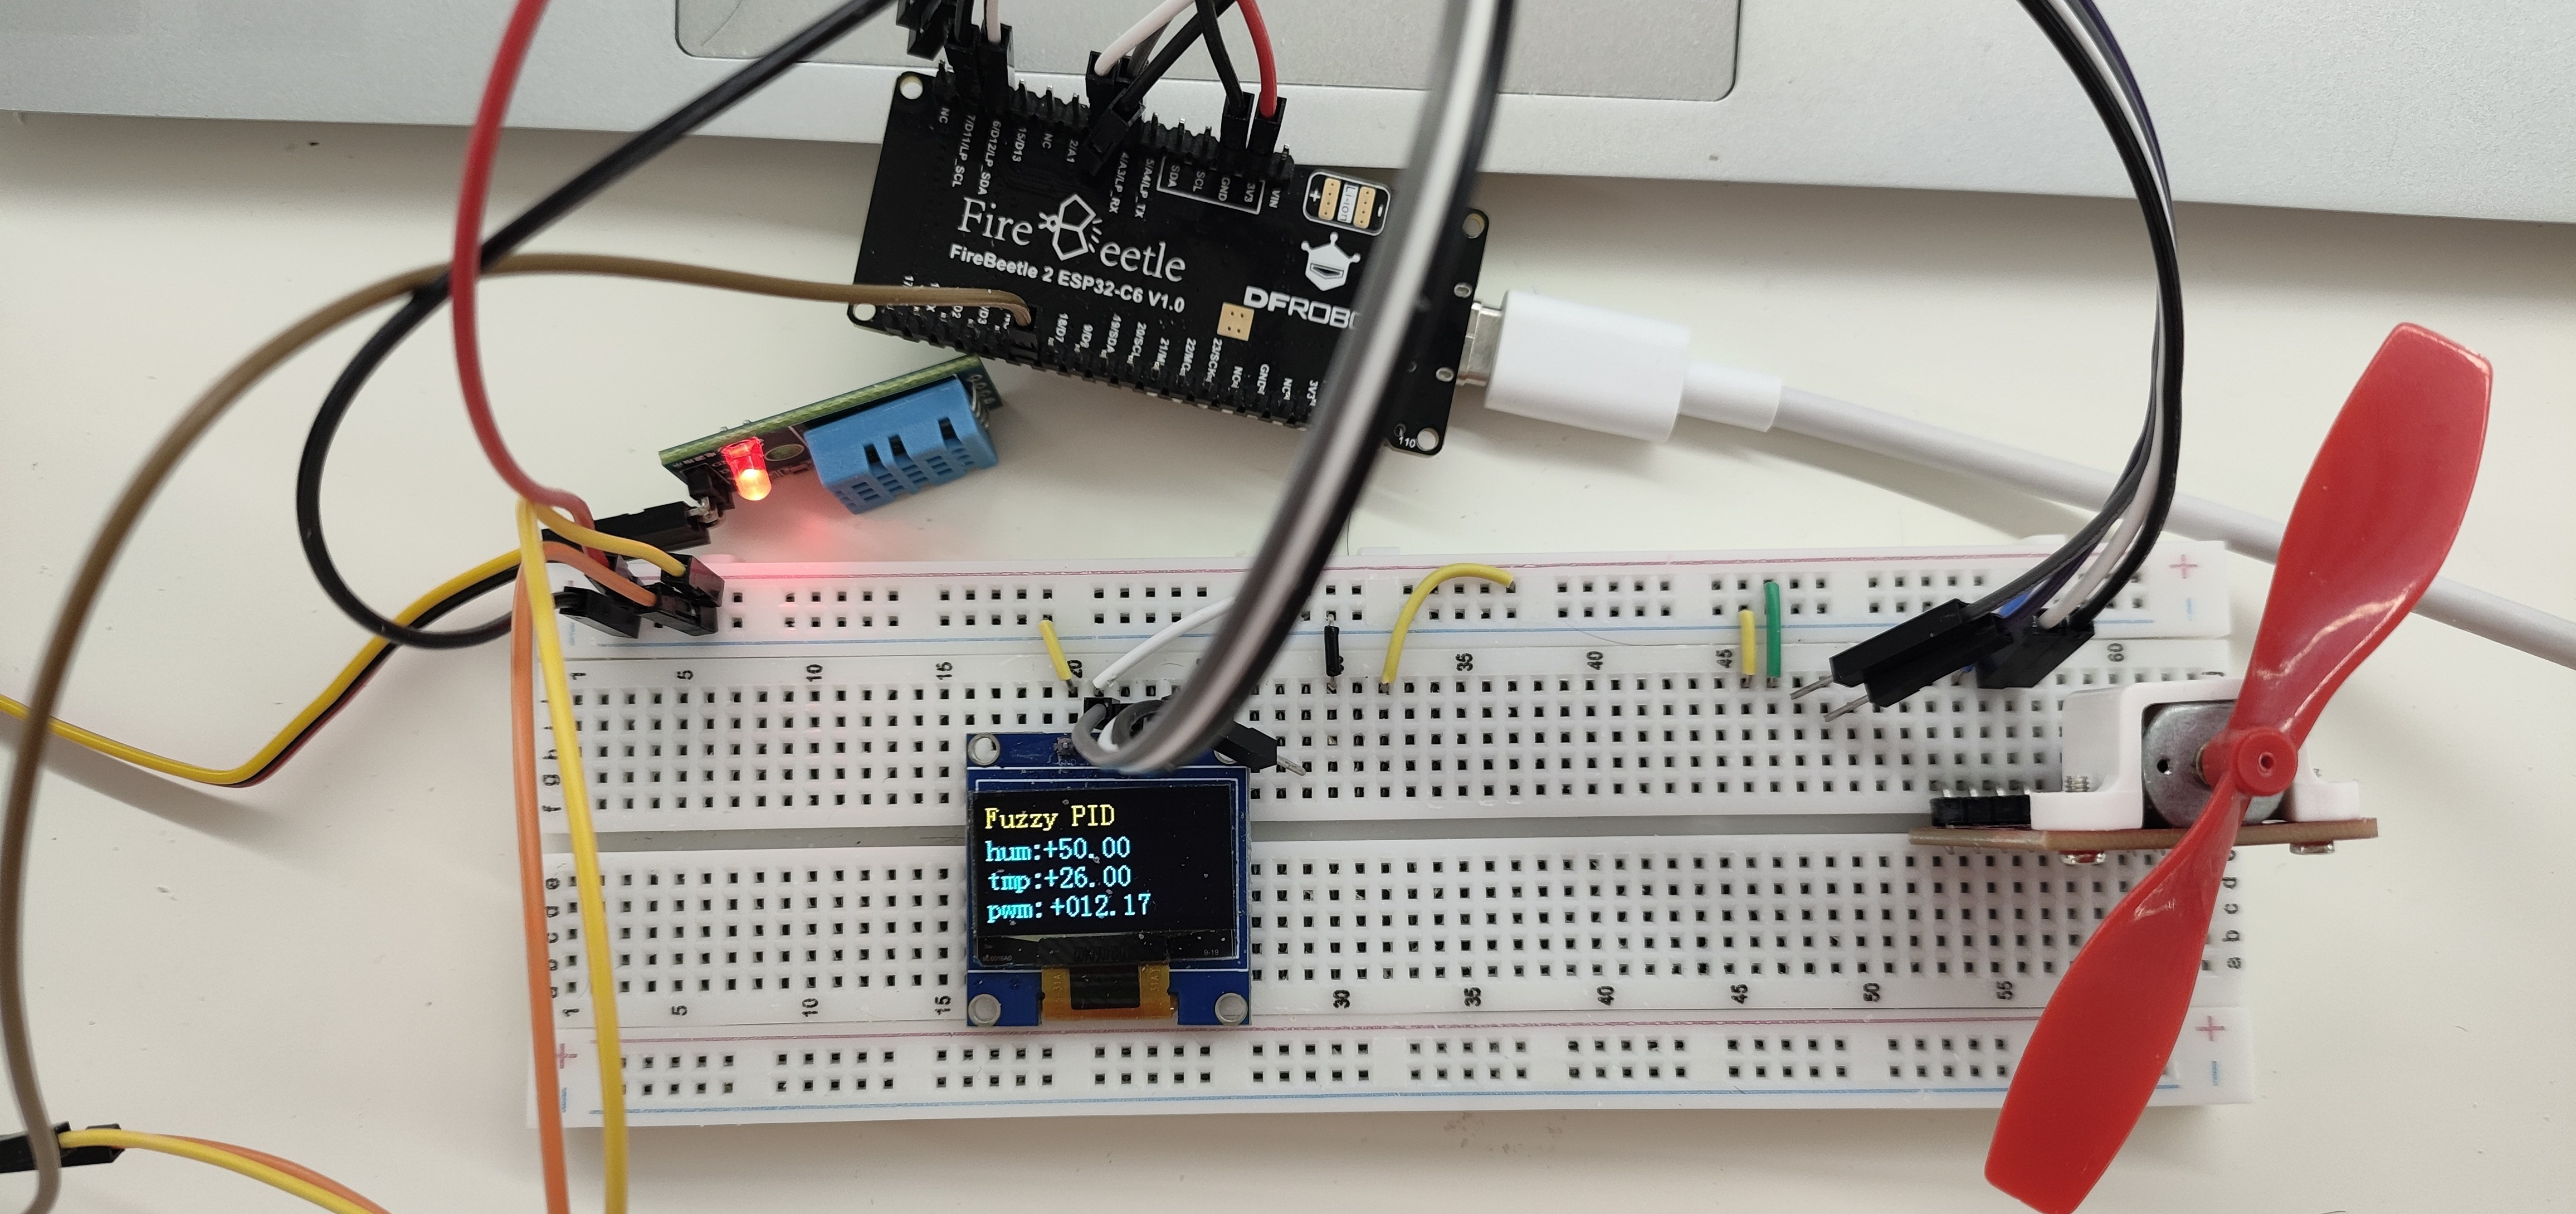
\includegraphics[width=0.85\linewidth]{figure/c}
			\caption{硬件接线实物图} % 图片标题
			\label{fig:image9} % 图片标签,用于在文中引用
		\end{figure}
		\item 测试过程中的 $delta\_kp$,$delta\_ki$,$delta\_kd$ 变化趋势:
		\begin{figure}[htbp]
			\centering
			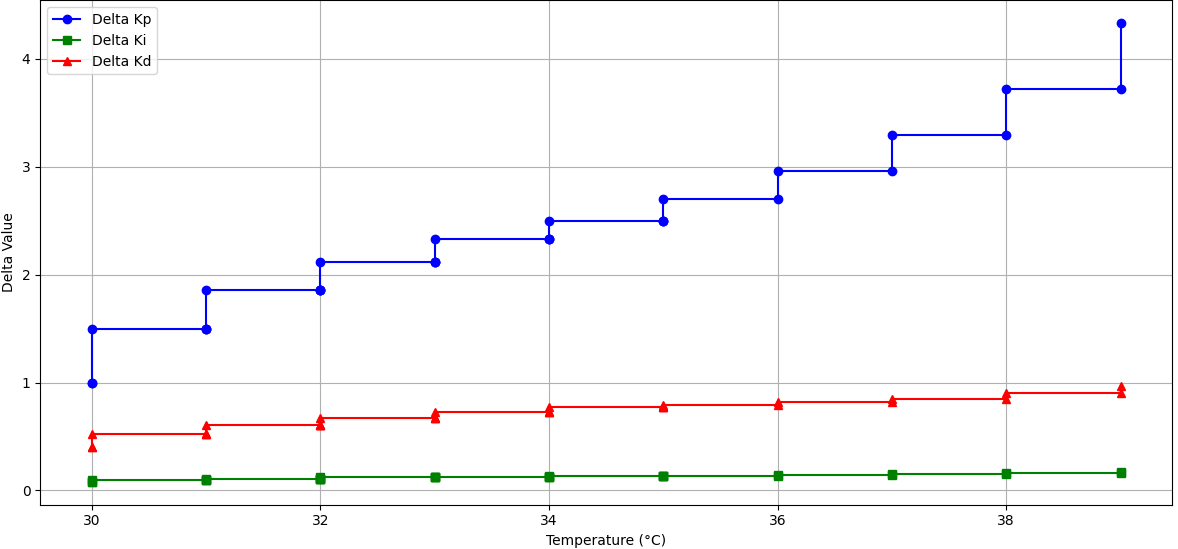
\includegraphics[width=0.85\linewidth]{figure/vs}
			\caption{控制变量的变化趋势}
			\label{fig:bianhua}
		\end{figure}
		\item 控制过程中的温度与输出的拟合直线较比模糊控制更加的平滑:
		\newpage
		\begin{figure}[htbp]
			\centering
			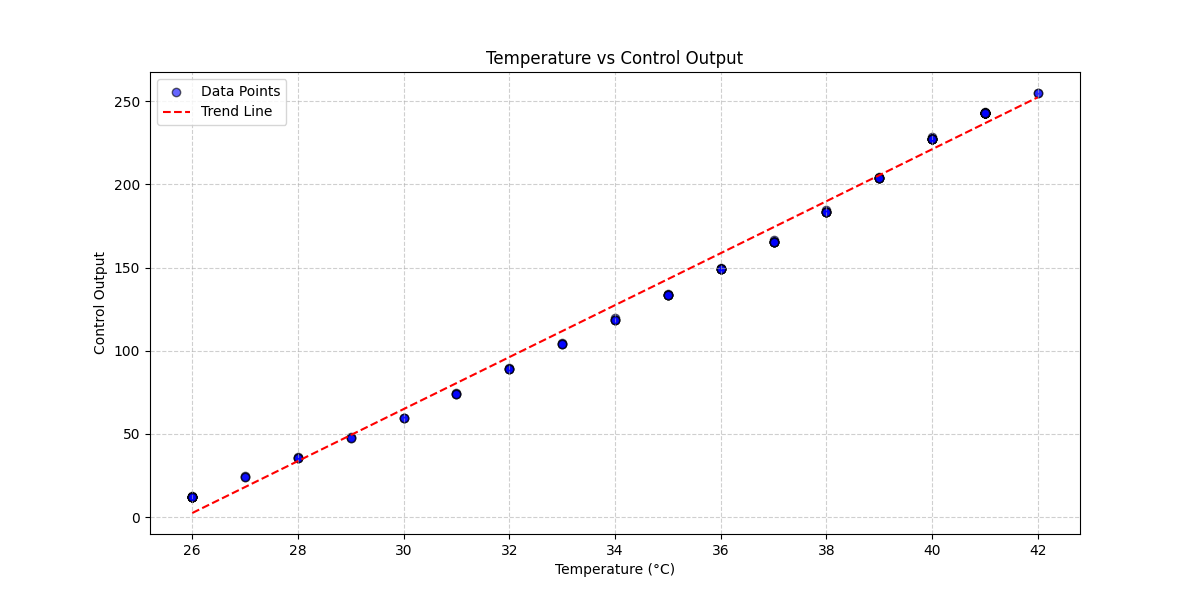
\includegraphics[width=1\linewidth]{figure/fuzzypid}
			\caption{温度与控制输出的效果图}
			\label{fig:hua}
		\end{figure}
		\item 实验最终测试效果图\newpage
				\begin{figure}[htbp]
					\centering
					\begin{subfigure}[t]{1\textwidth}
						\centering
						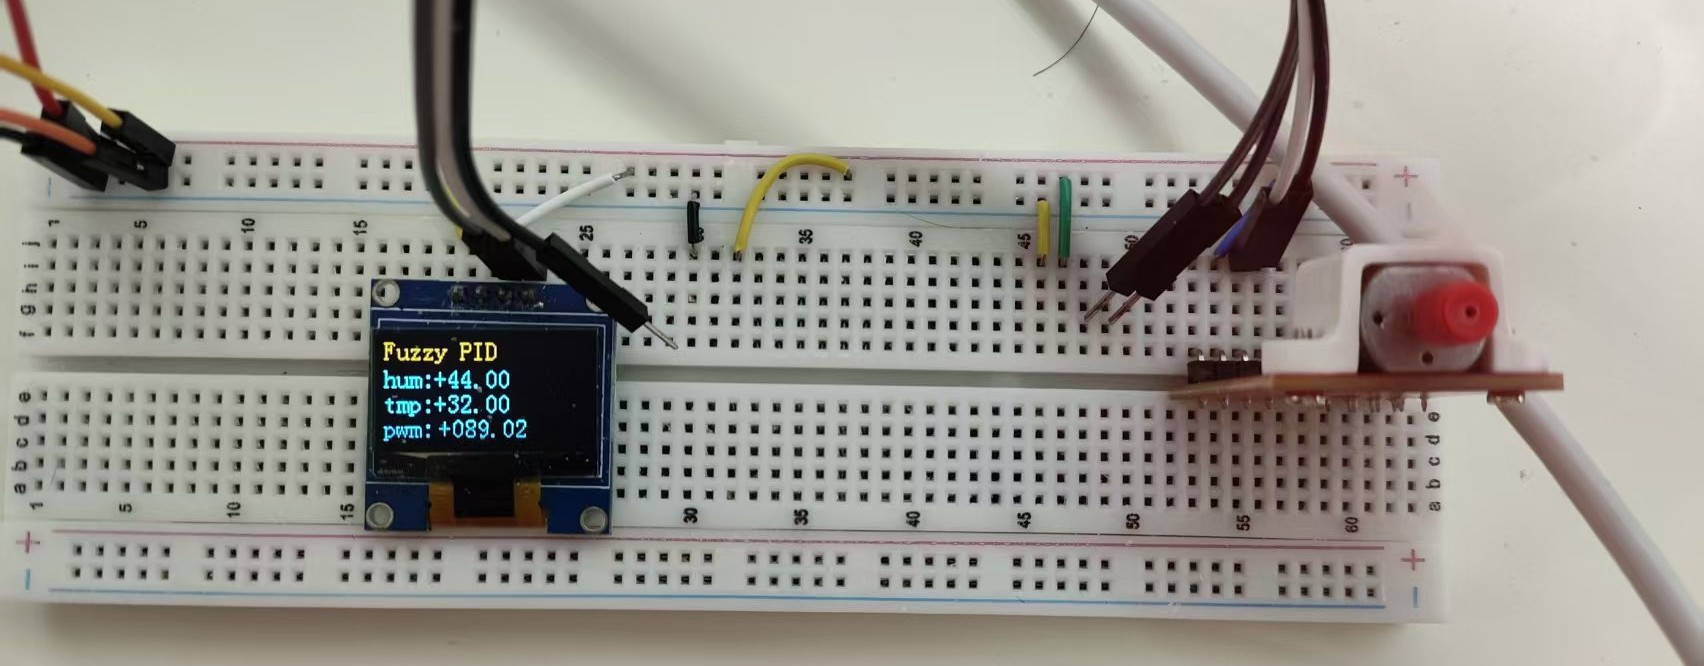
\includegraphics[width=0.55\linewidth]{figure/s}
						\caption{温度32℃效果图}
						\label{fig:z0}
					\end{subfigure}
					\begin{subfigure}[t]{1\textwidth}
						\centering
						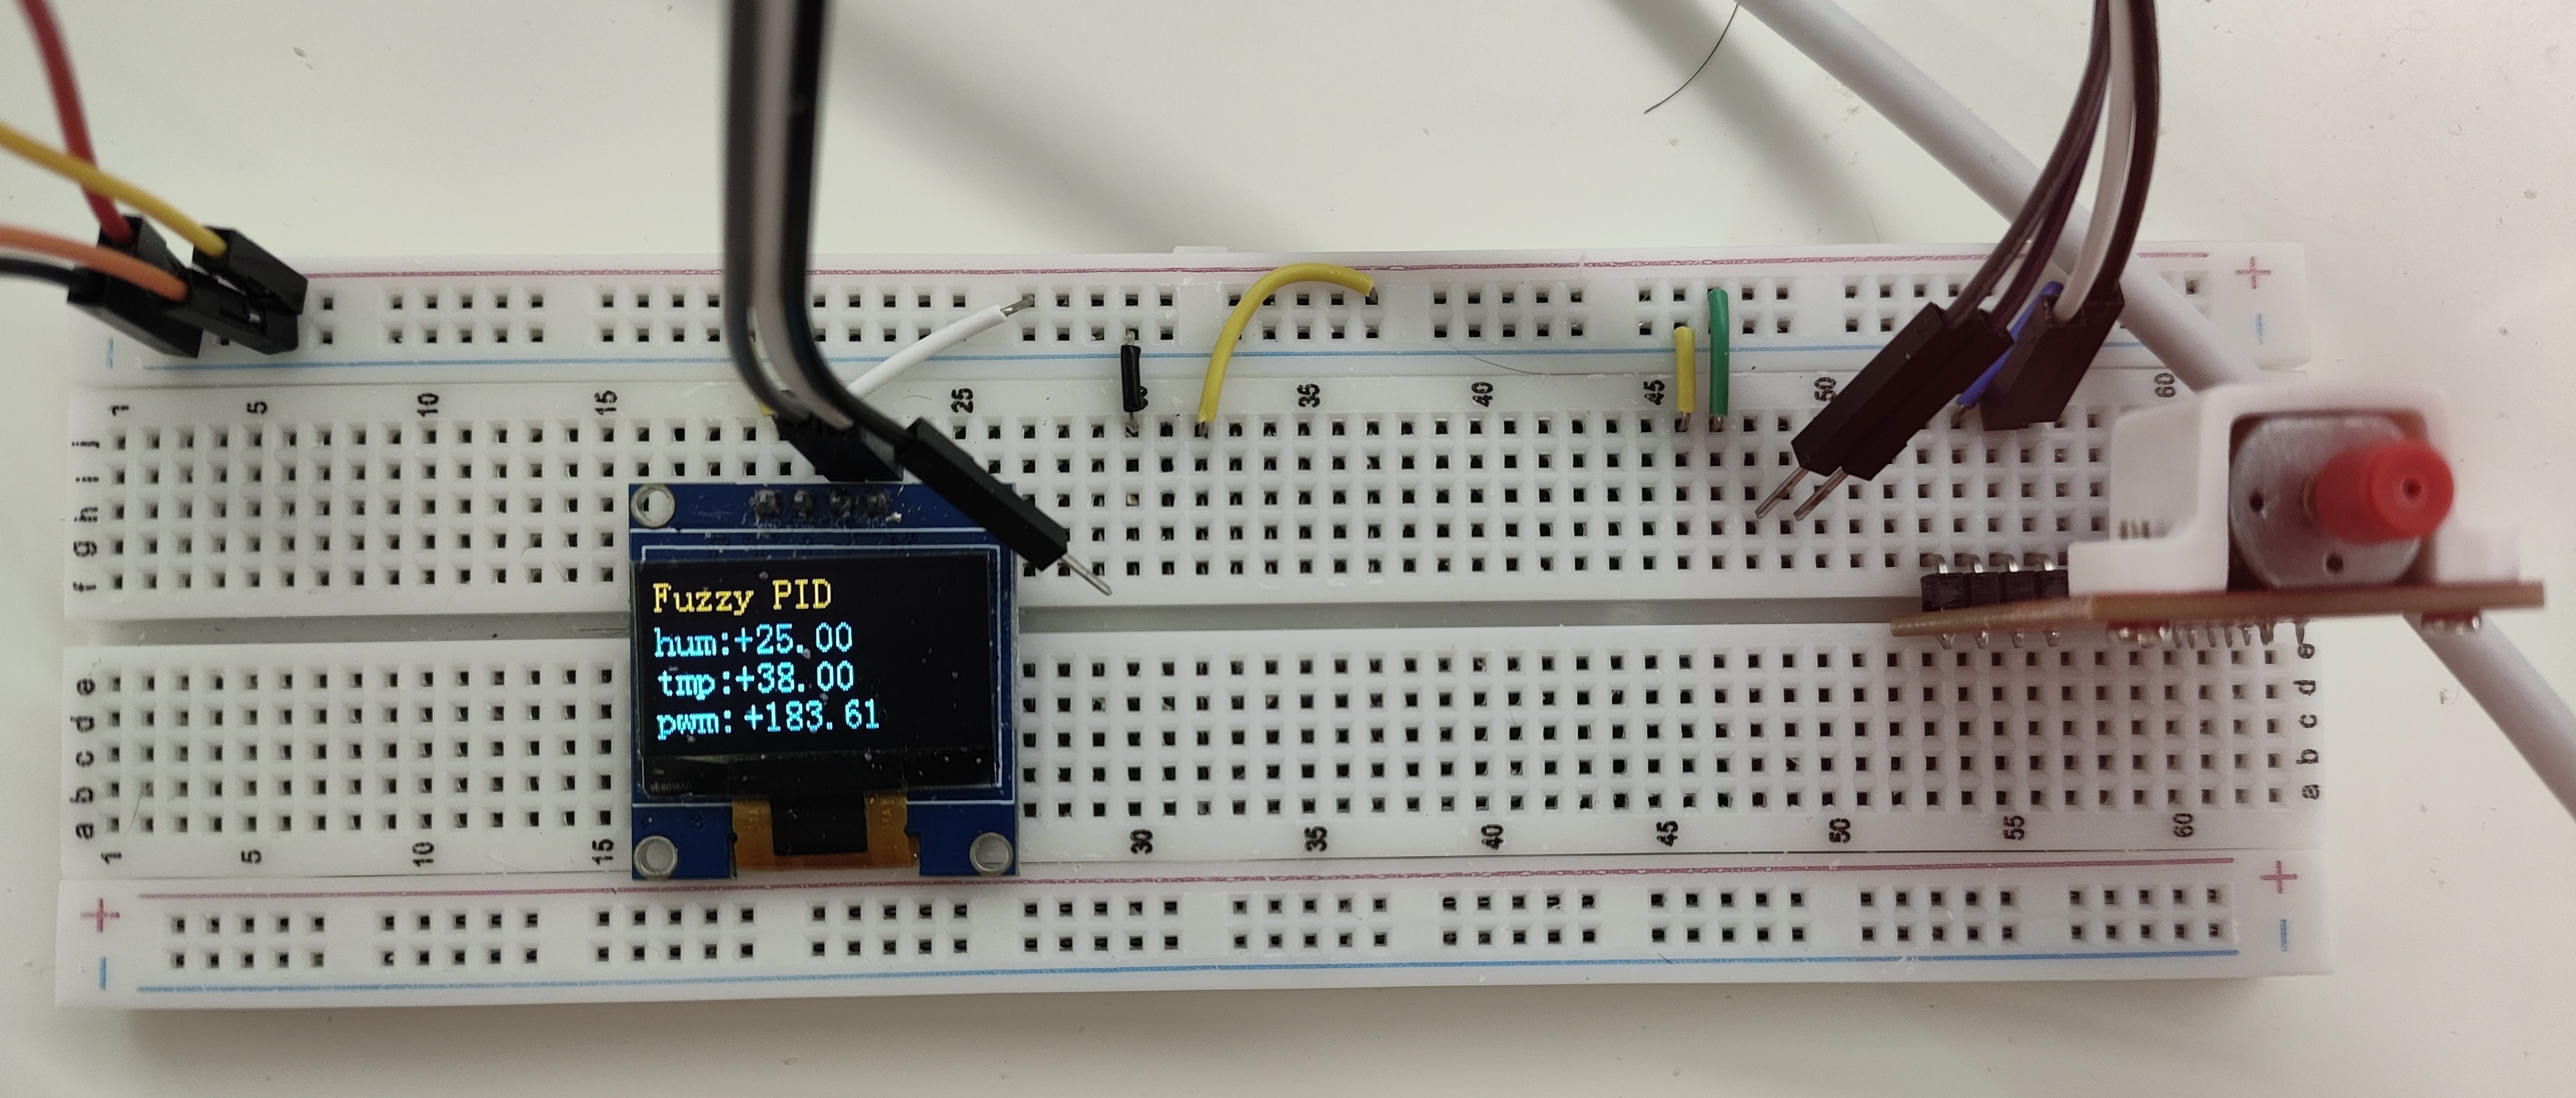
\includegraphics[width=0.55\linewidth]{figure/m}
						\caption{温度38℃效果图}
						\label{fig:z2}
					\end{subfigure}
					\begin{subfigure}[t]{1\textwidth}
						\centering
						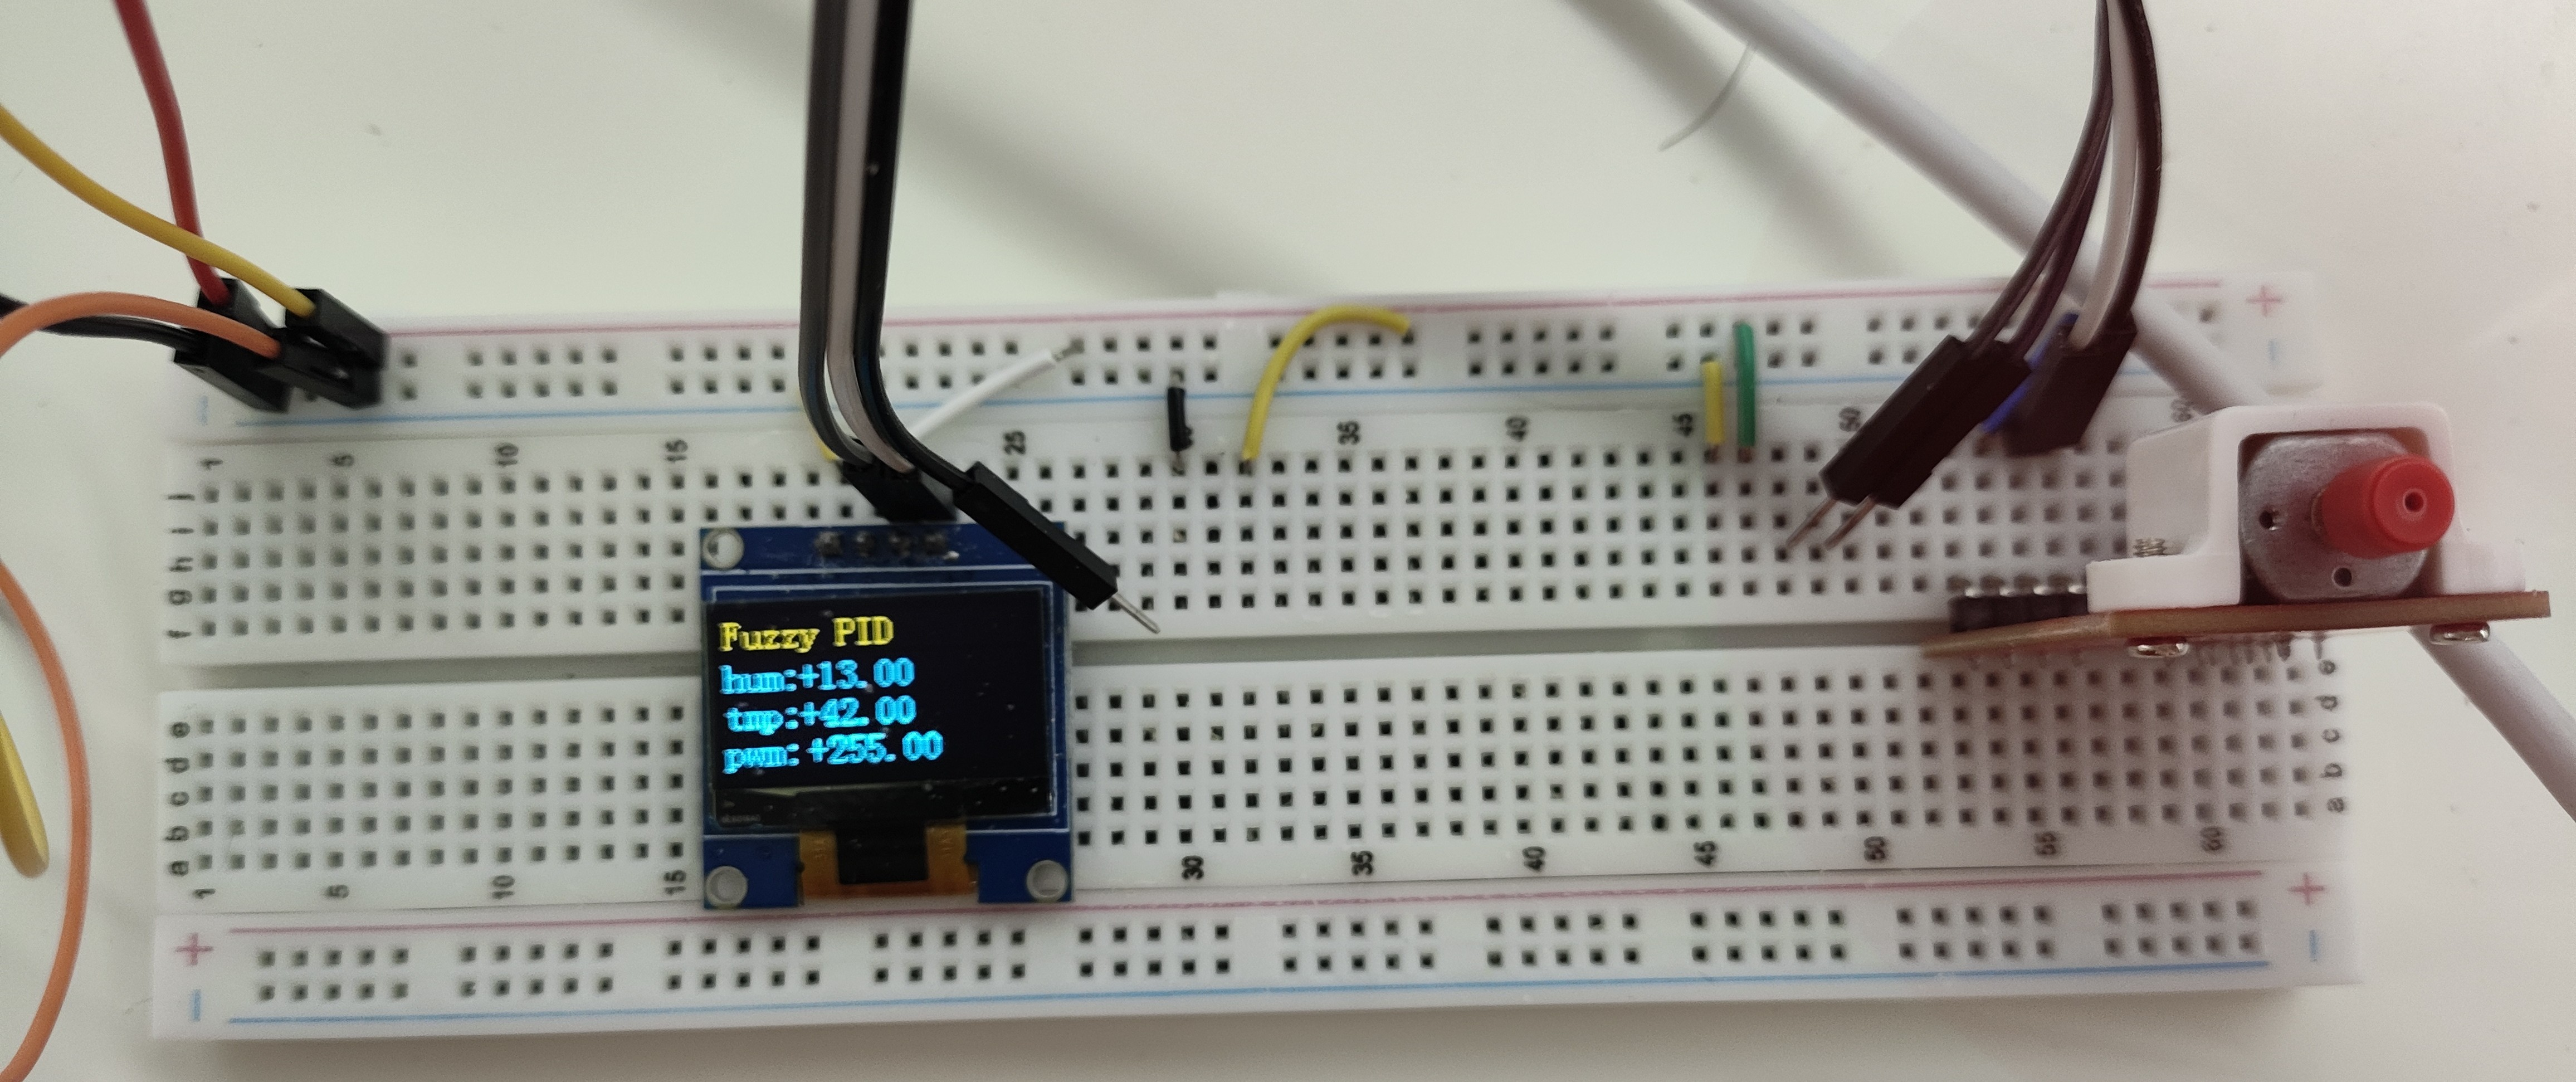
\includegraphics[width=0.55\linewidth]{figure/h}
						\caption{温度42℃效果图}
						\label{fig:z3}
					\end{subfigure}
				\end{figure}
	\end{itemize}
	
\section{实验思考与总结}
通过本次物联网控制技术实验,我深入理解并实践了基于Mamdani模糊控制算法的温湿度控制系统设计。实验不仅巩固了我对ESP32开发环境、FreeRTOS多任务编程、DHT11温湿度传感器数据采集、OLED屏幕数据显示以及L9110H电机驱动模块应用的理论知识,而且提升了我的实际操作能力和问题解决能力。
\begin{itemize}
	\item 实验收获
	\begin{enumerate}
		\item 理论知识与实践结合:通过亲自动手搭建 ESP32 开发环境,我更深入地理解了嵌入式系统开发的复杂性和细节。在实验过程中,我将课堂上学到的关于物联网控制技术的理论知识,如传感器数据采集、PID 控制原理、模糊控制算法等,应用到实际的温控风扇系统开发中。例如,我利用 DHT11 传感器采集温湿度数据,这让我明白了传感器的工作原理和数据处理方式。同时,我将模糊控制算法与 PID 控制相结合,实现了对风扇转速的智能调节,这让我深刻体会到理论知识在解决实际问题中的重要作用。
		\item 多任务编程技能提升:在 FreeRTOS 环境下进行多任务编程,是我在这次实验中的一个重要收获。我学会了如何合理地创建和管理任务,例如创建了模糊 PID 控制任务来周期性地读取温度数据、计算控制输出并驱动风扇电机。通过设置任务的优先级和堆栈大小,我确保了系统能够高效地运行多个任务,而不会出现任务抢占或资源冲突的问题。
		\item 传感器数据处理能力增强:通过使用DHT11温湿度传感器进行数据采集,我学会了如何处理和分析传感器数据,这对于进行环境监测和智能控制应用至关重要。
		\item 模糊控制算法应用:实验中实现的模糊 PID 控制算法,让我掌握了模糊逻辑在复杂系统控制中的应用。模糊控制能够处理系统中的不确定性,通过模糊规则库对输入变量进行模糊推理,从而得到合适的控制输出。在温控风扇系统中,模糊控制可以根据温度误差及其变化率动态调整 PID 参数,使系统具有更好的鲁棒性和适应性。这让我认识到模糊控制算法在实际应用中的强大功能,尤其是在面对非线性、时变性强的系统时,能够有效地提高控制效果。
	\end{enumerate}
	\item 实验反思
	\begin{enumerate}
		\item 系统稳定性问题:在实验过程中,我遇到了系统稳定性问题,这提示我在系统设计时需要更加关注硬件选择和软件优化,以确保系统的稳定运行。
		\item 算法优化空间:虽然模糊 PID 控制算法在本次实验中取得了良好的效果,但我也意识到算法还有进一步优化的空间,例如通过调整隶属度函数和规则库来提高控制精度。同时,我也可以考虑引入增量型 PID 控制方式,以更快速地响应系统的变化,进一步提升控制效果。
		\item 系统集成挑战:在将各个功能模块集成到一个系统中时,我遇到了一些挑战,这让我认识到在复杂系统设计中,模块化设计和接口标准化的重要性。
	\end{enumerate}
\end{itemize}

\newpage
\begin{appendices}
\section{主程序}
\begin{lstlisting}[language=C, caption={main.c}]
	#include <stdio.h>
	#include "freertos/FreeRTOS.h"
	#include "freertos/task.h"
	#include "OLED.h"
	#include "dht.h"
	#include "esp_log.h"
	#include <driver/gpio.h>
	#include <driver/ledc.h>
	#include "TMF.h"
	#include "mydht11.h"
	#include <pid_ctrl.h>
	#include "esp_spiffs.h"
	
	#define OLED_I2C I2C_NUM_0
	#define OLED_SCL 4
	#define OLED_SDA 3
	#define OLED_ADD 0x78
	#define OLED_SPEED 400000
	#define DHT_SENSOR_PIN 1
	#define DHT_SENSOR_TYPE DHT_TYPE_DHT11
	#define DELAY_TIME 3000
	
	static const char *TAG = "OLED_DHT";
	#define TAG1 "PID_TEST"
	
	float target_temperature = 25.0; // 目标温度
	
	// 显示温湿度数据
	void display_temp_hum(float temperature, float humidity, float output)
	{
		OLED_Clear();
		OLED_ShowString(0, 0, "Fuzzy PID", OLED_8X16);
		OLED_ShowString(0, 16, "hum:", OLED_8X16);
		OLED_ShowString(0, 32, "tmp:", OLED_8X16);
		OLED_ShowString(0, 48, "pwm:", OLED_8X16);
		OLED_ShowFloatNum(32, 16, humidity, 2, 2, OLED_8X16);
		OLED_ShowFloatNum(32, 32, temperature, 2, 2, OLED_8X16);
		OLED_ShowFloatNum(35, 48, output, 3, 2, OLED_8X16);
		OLED_Update();
	}
	
	void display_temp_humt(float temperature, float humidity)
	{
		OLED_Clear();
		OLED_ShowString(0, 16, "hum:", OLED_8X16);
		OLED_ShowString(0, 32, "tmp:", OLED_8X16);
		OLED_ShowFloatNum(32, 16, humidity, 2, 2, OLED_8X16);
		OLED_ShowFloatNum(32, 32, temperature, 2, 2, OLED_8X16);
		OLED_Update();
	}
	
	void fuzzy_control_task(void *pvParameter)
	{
		float current_temperature = 0.0;
		float humidity = 0.0;
		static float last_error = 0.0;
		
		while (1)
		{
			// 读取温湿度数据
			esp_err_t result = dht_read_float_data(DHT_SENSOR_TYPE,
			DHT_SENSOR_PIN, &humidity, &current_temperature);
			if (result == ESP_OK)
			{
				// 计算误差和误差变化
				float error = target_temperature - current_temperature;
				float delta_error = error - last_error;
				
				// 模糊化
				FuzzyMembership error_membership = fuzzify_error(error);
				FuzzyMembership delta_error_membership = fuzzify_delta_error(delta_error);
				
				// 模糊推理
				FuzzyMembership control_membership = infer_control(error_membership,
				delta_error_membership);
				
				// 去模糊化
				float control_output = defuzzify(control_membership);
				
				// 更新上一次误差
				last_error = error;
				
				// 显示温湿度和控制输出
				display_temp_hum(current_temperature, humidity, control_output);
				ESP_LOGI(TAG,
				"Temp: %.1f, Hum: %.1f, Error: %.1f,Delta Error: %.1f, Control Output: %.1f",
				current_temperature, humidity, error, delta_error, control_output);
				
				set_motor_speed((int)control_output);
			}
			else
			{
				ESP_LOGE(TAG, "Failed to read data from DHT sensor: %s",
				esp_err_to_name(result));
				OLED_Clear();
				OLED_ShowString(0, 0, "Sensor Error", OLED_8X16);
				OLED_Update();
			}
			
			vTaskDelay(pdMS_TO_TICKS(1000));
		}
		
	}
	
	void init_spiffs()
	{
		esp_vfs_spiffs_conf_t conf = {
			.base_path = "/spiffs",
			.partition_label = NULL,
			.max_files = 5,
			.format_if_mount_failed = true};
		
		esp_err_t ret = esp_vfs_spiffs_register(&conf);
		
		if (ret != ESP_OK)
		{
			ESP_LOGE(TAG, "Failed to mount SPIFFS (%s)", esp_err_to_name(ret));
		}
		else
		{
			ESP_LOGI(TAG, "SPIFFS mounted successfully");
		}
	}
	
	void fuzzy_pid_task(void *pvParameter){
		float current_temp = 0.0;
		float hum = 0.0;
		static float last_error = 0.0;
		pid_ctrl_block_handle_t pid;
		
		// 初始化PID控制器
		pid_ctrl_config_t pid_config = {
			.init_param = {
				.kp = 10.8,          // 比例增益
				.ki = 0.1,           // 积分增益(适当增大以消除稳态误差)
				.kd = 0.06,          // 微分增益(适当增大以减少振荡)
				.max_output = 255.0, // 限制最大输出为255
				.min_output = 0.0,
				.max_integral = 2.0,
				.min_integral = -2.0,
				.cal_type = PID_CAL_TYPE_POSITIONAL}};
		if (pid_new_control_block(&pid_config, &pid) != ESP_OK)
		{
			ESP_LOGE(TAG1, "Failed to create PID control block");
			vTaskDelete(NULL);
		}
		
		while(1){
			esp_err_t result = dht_read_float_data(DHT_SENSOR_TYPE,DHT_SENSOR_PIN,&hum,&current_temp);
			
			if(result == ESP_OK){
				float error = current_temp - target_temperature;
				float delta_error = error - last_error;
				//模糊化
				FuzzyMembership error_memb = fuzzify_error(error);
				FuzzyMembership delta_error_memb = fuzzify_delta_error(delta_error);
				
				//模糊推理
				float delta_kp,delta_ki,delta_kd;
				infer_pid(error_memb,delta_error_memb,&delta_kp,&delta_ki,&delta_kd);
				// 更新PID参数
				pid_ctrl_parameter_t new_params;
				new_params.kp = pid_config.init_param.kp + delta_kp;
				new_params.ki = pid_config.init_param.ki + delta_ki;
				new_params.kd = pid_config.init_param.kd + delta_kd;
				new_params.max_output = pid_config.init_param.max_output;
				new_params.min_output = pid_config.init_param.min_output;
				new_params.max_integral = pid_config.init_param.max_integral;
				new_params.min_integral = pid_config.init_param.min_integral;
				new_params.cal_type = pid_config.init_param.cal_type;
				pid_update_parameters(pid, &new_params);
				ESP_LOGI(TAG1, "Delta Kp: %.2f, Delta Ki: %.2f, Delta Kd: %.2f", delta_kp, delta_ki, delta_kd);
				
				// 计算控制输出
				float control_output;
				if (pid_compute(pid, error, &control_output) == ESP_OK)
				{
					if (control_output > 255.0) control_output = 255.0;
					display_temp_hum(current_temp, hum, control_output);
					ESP_LOGI(TAG1, "Temp: %.2f, Hum: %.2f, Error: %.2f, Control Output: %.2f", current_temp, hum, error, control_output);
					if(delta_error != 0)
					set_motor_speed(control_output);
				}
				else ESP_LOGE(TAG1, "PID computation failed");
				last_error = error;
			}
			else
			{
				ESP_LOGE(TAG1, "Failed to read data from DHT sensor: %s",
				esp_err_to_name(result));
				OLED_Clear();
				OLED_ShowString(0, 0, "Sensor Error", OLED_8X16);
				OLED_Update();
			}
			vTaskDelay(pdMS_TO_TICKS(1500));
		}
		pid_del_control_block(pid);
	}

	void app_main(void)
	{
		l9110_pwm_init();
		OLED_Init(OLED_I2C, OLED_ADD, OLED_SCL, OLED_SDA, OLED_SPEED);
		// 设置 DHT11 引脚为上拉模式
		// gpio_set_pull_mode(DHT_SENSOR_PIN, GPIO_PULLUP_ONLY);
		
		// 创建模糊控制任务
		// xTaskCreate(fuzzy_control_task, "FuzzyControlTask", 4096, NULL, 5, NULL);
		// 创建PID控制任务
		xTaskCreate(fuzzy_pid_task, "FuzzyPIDTask", 4096, NULL, 5, NULL);
		
		// 创建Ziegler-Nichols调参任务
		// xTaskCreate(ziegler_nichols_tuning_task, "ZNTuningTask", 4096, NULL, 5, NULL);
	}
\end{lstlisting}
\newpage
\section{OLED显示代码}
\begin{lstlisting}[language=C, caption=OLED.c]
#include "OLED.h"
uint8_t OLED_DisplayBuf[8][128];

//I2C总线句柄
i2c_master_bus_handle_t oled_bus_handle;

//OLED设备句柄
i2c_master_dev_handle_t oled_dev_handle;

/**
* 函    数:OLED写命令
* 参    数:Command 要写入的命令值,范围:0x00-0xFF
* 返 回 值:无
*/
void OLED_WriteCommand(uint8_t Command)
{
	uint8_t writebuffer[2];
	
	writebuffer[0] = 0x00;
	writebuffer[1] = Command;
	ESP_ERROR_CHECK(i2c_master_transmit(oled_dev_handle, writebuffer, 2, -1));
}

/**
* 函    数:OLED写数据
* 参    数:Data 要写入数据的起始地址
* 参    数:Count 要写入数据的数量
* 返 回 值:无
*/
void OLED_WriteData(uint8_t *Data, uint8_t Count)
{
	uint8_t i;
	uint8_t writebuffer[Count+1];
	
	writebuffer[0] = 0x40;
	
	for(i = 0; i<Count; i ++) writebuffer[i+1] = Data[i];
	ESP_ERROR_CHECK(i2c_master_transmit(oled_dev_handle,writebuffer,Count+1,-1));
}

/**
* 函    数:OLED初始化
* 参    数:port  I2C端口号
* 参    数:add   oled地址
* 参    数:scl   SCL引脚
* 参    数:sda   SDA引脚
* 参    数:speed SCL时钟频率(Hz),不应大于400k
* 返 回 值:无
* 说    明:使用前,需要调用此初始化函数
*/
void OLED_Init(int port, uint8_t add, int scl, int sda, int speed)
{
	//配置I2C总线
	i2c_master_bus_config_t oled_i2c_mst_cfg = 
	{
		.clk_source = I2C_CLK_SRC_DEFAULT,      //使用默认时钟源
		.i2c_port = port,                       //指定I2C端口号
		.scl_io_num = scl,                      //指定SCL引脚号
		.sda_io_num = sda,                      //指定SDA引脚号
		.glitch_ignore_cnt = 7,                 //设置毛刺忽略计数
		.flags.enable_internal_pullup = false,  //禁用内部上拉电阻
	};
	
	//创建I2C总线并获取句柄
	ESP_ERROR_CHECK(i2c_new_master_bus(&oled_i2c_mst_cfg, &oled_bus_handle));
	
	//配置I2C从机设备
	i2c_device_config_t oled_dev_cfg = 
	{
		.dev_addr_length = I2C_ADDR_BIT_LEN_7,  //设置设备地址长度为7位
		.device_address = add >> 1,             //指定设备地址
		.scl_speed_hz = speed,                  //设置I2C时钟速度
		.flags.disable_ack_check = false,       //启用ACK检查
	};
	
	//将设备添加到I2C总线并获取设备句柄
	ESP_ERROR_CHECK(i2c_master_bus_add_device(oled_bus_handle, &oled_dev_cfg, &oled_dev_handle));
	
	/*写入一系列的命令,对OLED进行初始化配置*/
	OLED_WriteCommand(0xAE);	//设置显示开启/关闭,0xAE关闭,0xAF开启
	
	OLED_WriteCommand(0xD5);	//设置显示时钟分频比/振荡器频率
	OLED_WriteCommand(0x80);	//0x00-0xFF
	
	OLED_WriteCommand(0xA8);	//设置多路复用率
	OLED_WriteCommand(0x3F);	//0x0E-0x3F
	
	OLED_WriteCommand(0xD3);	//设置显示偏移
	OLED_WriteCommand(0x00);	//0x00-0x7F
	
	OLED_WriteCommand(0x40);	//设置显示开始行,0x40-0x7F
	
	OLED_WriteCommand(0xA1);	//设置左右方向,0xA1正常,0xA0左右反置
	
	OLED_WriteCommand(0xC8);	//设置上下方向,0xC8正常,0xC0上下反置
	
	OLED_WriteCommand(0xDA);	//设置COM引脚硬件配置
	OLED_WriteCommand(0x12);
	
	OLED_WriteCommand(0x81);	//设置对比度
	OLED_WriteCommand(0xCF);	//0x00-0xFF
	
	OLED_WriteCommand(0xD9);	//设置预充电周期
	OLED_WriteCommand(0xF1);
	
	OLED_WriteCommand(0xDB);	//设置VCOMH取消选择级别
	OLED_WriteCommand(0x30);
	
	OLED_WriteCommand(0xA4);	//设置整个显示打开/关闭
	
	OLED_WriteCommand(0xA6);	//设置正常/反色显示,0xA6正常,0xA7反色
	
	OLED_WriteCommand(0x8D);	//设置充电泵
	OLED_WriteCommand(0x14);
	
	OLED_WriteCommand(0xAF);	//开启显示
	
	OLED_Clear();				//清空显存数组
	OLED_Update();				//更新显示,清屏,防止初始化后未显示内容时花屏
}

/**
* 函    数:OLED设置显示光标位置
* 参    数:Page 指定光标所在的页,范围:0-7
* 参    数:X 指定光标所在的X轴坐标,范围:0-127
* 返 回 值:无
* 说    明:OLED默认的Y轴,只能8个Bit为一组写入,即1页等于8个Y轴坐标
*/
void OLED_SetCursor(uint8_t Page, uint8_t X)
{
	/*如果使用此程序驱动1.3寸的OLED显示屏,则需要解除此注释*/
	/*因为1.3寸的OLED驱动芯片(SH1106)有132列*/
	/*屏幕的起始列接在了第2列,而不是第0列*/
	/*所以需要将X加2,才能正常显示*/
	//	X += 2;
	
	/*通过指令设置页地址和列地址*/
	OLED_WriteCommand(0xB0 | Page);					//设置页位置
	OLED_WriteCommand(0x10 | ((X & 0xF0) >> 4));	//设置X位置高4位
	OLED_WriteCommand(0x00 | (X & 0x0F));			//设置X位置低4位
}

/**
* 函    数:次方函数
* 参    数:X 底数
* 参    数:Y 指数
* 返 回 值:等于X的Y次方
*/
uint32_t OLED_Pow(uint32_t X, uint32_t Y)
{
	uint32_t Result = 1;	//结果默认为1
	while (Y --)			//累乘Y次
	{
		Result *= X;		//每次把X累乘到结果上
	}
	return Result;
}

/**
* 函    数:判断指定点是否在指定多边形内部
* 参    数:nvert 多边形的顶点数
* 参    数:vertx verty 包含多边形顶点的x和y坐标的数组
* 参    数:testx testy 测试点的X和y坐标
* 返 回 值:指定点是否在指定多边形内部,1:在内部,0:不在内部
*/
uint8_t OLED_pnpoly(uint8_t nvert, int16_t *vertx, int16_t *verty, int16_t testx, int16_t testy)
{
	int16_t i, j, c = 0;
	
	for (i = 0, j = nvert - 1; i < nvert; j = i++)
	{
		if (((verty[i] > testy) != (verty[j] > testy)) &&
		(testx < (vertx[j] - vertx[i]) * (testy - verty[i]) / (verty[j] - verty[i]) + vertx[i])) c = !c;
	}
	return c;
}

/**
* 函    数:判断指定点是否在指定角度内部
* 参    数:X Y 指定点的坐标
* 参    数:StartAngle EndAngle 起始角度和终止角度,范围:-180-180
*           水平向右为0度,水平向左为180度或-180度,下方为正数,上方为负数,顺时针旋转
* 返 回 值:指定点是否在指定角度内部,1:在内部,0:不在内部
*/
uint8_t OLED_IsInAngle(int16_t X, int16_t Y, int16_t StartAngle, int16_t EndAngle)
{
	int16_t PointAngle;
	PointAngle = atan2(Y, X) / 3.14 * 180;	//计算指定点的弧度,并转换为角度表示
	if (StartAngle < EndAngle)	//起始角度小于终止角度的情况
	{
		/*如果指定角度在起始终止角度之间,则判定指定点在指定角度*/
		if (PointAngle >= StartAngle && PointAngle <= EndAngle) return 1;
	}
	else			//起始角度大于于终止角度的情况
	{
		/*如果指定角度大于起始角度或者小于终止角度,则判定指定点在指定角度*/
		if (PointAngle >= StartAngle || PointAngle <= EndAngle) return 1;
	}
	return 0;		//不满足以上条件,则判断判定指定点不在指定角度
}


/**
* 函    数:将OLED显存数组更新到OLED屏幕
* 参    数:无
* 返 回 值:无
* 说    明:所有的显示函数,都只是对OLED显存数组进行读写
*           随后调用OLED_Update函数或OLED_UpdateArea函数
*           才会将显存数组的数据发送到OLED硬件,进行显示
*           故调用显示函数后,要想真正地呈现在屏幕上,还需调用更新函数
*/
void OLED_Update(void)
{
	uint8_t j;
	/*遍历每一页*/
	for (j = 0; j < 8; j ++)
	{
		/*设置光标位置为每一页的第一列*/
		OLED_SetCursor(j, 0);
		/*连续写入128个数据,将显存数组的数据写入到OLED硬件*/
		OLED_WriteData(OLED_DisplayBuf[j], 128);
	}
}

/**
* 函    数:将OLED显存数组部分更新到OLED屏幕
* 参    数:X 指定区域左上角的横坐标,范围:-32768-32767,屏幕区域:0-127
* 参    数:Y 指定区域左上角的纵坐标,范围:-32768-32767,屏幕区域:0-63
* 参    数:Width 指定区域的宽度,范围:0-128
* 参    数:Height 指定区域的高度,范围:0-64
* 返 回 值:无
* 说    明:此函数会至少更新参数指定的区域
*           如果更新区域Y轴只包含部分页,则同一页的剩余部分会跟随一起更新
* 说    明:所有的显示函数,都只是对OLED显存数组进行读写
*           随后调用OLED_Update函数或OLED_UpdateArea函数
*           才会将显存数组的数据发送到OLED硬件,进行显示
*           故调用显示函数后,要想真正地呈现在屏幕上,还需调用更新函数
*/
void OLED_UpdateArea(int16_t X, int16_t Y, uint8_t Width, uint8_t Height)
{
	int16_t j;
	int16_t Page, Page1;
	
	/*负数坐标在计算页地址时需要加一个偏移*/
	/*(Y + Height - 1) / 8 + 1的目的是(Y + Height) / 8并向上取整*/
	Page = Y / 8;
	Page1 = (Y + Height - 1) / 8 + 1;
	if (Y < 0)
	{
		Page -= 1;
		Page1 -= 1;
	}
	
	/*遍历指定区域涉及的相关页*/
	for (j = Page; j < Page1; j ++)
	{
		if (X >= 0 && X <= 127 && j >= 0 && j <= 7)		//超出屏幕的内容不显示
		{
			/*设置光标位置为相关页的指定列*/
			OLED_SetCursor(j, X);
			/*连续写入Width个数据,将显存数组的数据写入到OLED硬件*/
			OLED_WriteData(&OLED_DisplayBuf[j][X], Width);
		}
	}
}

/**
* 函    数:将OLED显存数组全部清零
* 参    数:无
* 返 回 值:无
* 说    明:调用此函数后,要想真正地呈现在屏幕上,还需调用更新函数
*/
void OLED_Clear(void)
{
	uint8_t i, j;
	for (j = 0; j < 8; j ++)				//遍历8页
	{
		for (i = 0; i < 128; i ++)			//遍历128列
		{
			OLED_DisplayBuf[j][i] = 0x00;	//将显存数组数据全部清零
		}
	}
}

/**
* 函    数:将OLED显存数组部分清零
* 参    数:X 指定区域左上角的横坐标,范围:-32768-32767,屏幕区域:0-127
* 参    数:Y 指定区域左上角的纵坐标,范围:-32768-32767,屏幕区域:0-63
* 参    数:Width 指定区域的宽度,范围:0-128
* 参    数:Height 指定区域的高度,范围:0-64
* 返 回 值:无
* 说    明:调用此函数后,要想真正地呈现在屏幕上,还需调用更新函数
*/
void OLED_ClearArea(int16_t X, int16_t Y, uint8_t Width, uint8_t Height)
{
	int16_t i, j;
	for (j = Y; j < Y + Height; j ++)		//遍历指定页
		for (i = X; i < X + Width; i ++)	//遍历指定列
	      if (i >= 0 && i <= 127 && j >=0 && j <= 63)	
			OLED_DisplayBuf[j / 8][i] &= ~(0x01 << (j % 8));
}

/**
* 函    数:将OLED显存数组全部取反
* 参    数:无
* 返 回 值:无
* 说    明:调用此函数后,要想真正地呈现在屏幕上,还需调用更新函数
*/
void OLED_Reverse(void)
{
	uint8_t i, j;
	for (j = 0; j < 8; j ++)				//遍历8页
	{
		for (i = 0; i < 128; i ++)			//遍历128列
		{
			OLED_DisplayBuf[j][i] ^= 0xFF;	//将显存数组数据全部取反
		}
	}
}

/**
* 函    数:将OLED显存数组部分取反
* 参    数:X 指定区域左上角的横坐标,范围:-32768-32767,屏幕区域:0-127
* 参    数:Y 指定区域左上角的纵坐标,范围:-32768-32767,屏幕区域:0-63
* 参    数:Width 指定区域的宽度,范围:0-128
* 参    数:Height 指定区域的高度,范围:0-64
* 返 回 值:无
* 说    明:调用此函数后,要想真正地呈现在屏幕上,还需调用更新函数
*/
void OLED_ReverseArea(int16_t X, int16_t Y, uint8_t Width, uint8_t Height)
{
	int16_t i, j;
	
	for (j = Y; j < Y + Height; j ++)		//遍历指定页
	{
		for (i = X; i < X + Width; i ++)	//遍历指定列
		{
			if (i >= 0 && i <= 127 && j >=0 && j <= 63)			//超出屏幕的内容不显示
			{
				OLED_DisplayBuf[j / 8][i] ^= 0x01 << (j % 8);	//将显存数组指定数据取反
			}
		}
	}
}

/**
* 函    数:OLED显示一个字符
* 参    数:X 指定字符左上角的横坐标,范围:-32768-32767,屏幕区域:0-127
* 参    数:Y 指定字符左上角的纵坐标,范围:-32768-32767,屏幕区域:0-63
* 参    数:Char 指定要显示的字符,范围:ASCII码可见字符
* 参    数:FontSize 指定字体大小
*           范围:OLED_8X16		宽8像素,高16像素
*                 OLED_6X8		宽6像素,高8像素
* 返 回 值:无
* 说    明:调用此函数后,要想真正地呈现在屏幕上,还需调用更新函数
*/
void OLED_ShowChar(int16_t X, int16_t Y, char Char, uint8_t FontSize)
{
	if (FontSize == OLED_8X16)		//字体为宽8像素,高16像素
	{
		/*将ASCII字模库OLED_F8x16的指定数据以8*16的图像格式显示*/
		OLED_ShowImage(X, Y, 8, 16, OLED_F8x16[Char - ' ']);
	}
	else if(FontSize == OLED_6X8)	//字体为宽6像素,高8像素
	{
		/*将ASCII字模库OLED_F6x8的指定数据以6*8的图像格式显示*/
		OLED_ShowImage(X, Y, 6, 8, OLED_F6x8[Char - ' ']);
	}
}

/**
* 函    数:OLED显示字符串
* 参    数:X 指定字符串左上角的横坐标,范围:-32768-32767,屏幕区域:0-127
* 参    数:Y 指定字符串左上角的纵坐标,范围:-32768-32767,屏幕区域:0-63
* 参    数:String 指定要显示的字符串,范围:ASCII码可见字符组成的字符串
* 参    数:FontSize 指定字体大小
*           范围:OLED_8X16		宽8像素,高16像素
*                 OLED_6X8		宽6像素,高8像素
* 返 回 值:无
* 说    明:调用此函数后,要想真正地呈现在屏幕上,还需调用更新函数
*/
void OLED_ShowString(int16_t X, int16_t Y, char *String, uint8_t FontSize)
{
	uint8_t i;
	for (i = 0; String[i] != '\0'; i++)		//遍历字符串的每个字符
	{
		/*调用OLED_ShowChar函数,依次显示每个字符*/
		OLED_ShowChar(X + i * FontSize, Y, String[i], FontSize);
	}
}

void OLED_ShowNum(int16_t X, int16_t Y, uint32_t Number, uint8_t Length, uint8_t FontSize)
{
	uint8_t i;
	for (i = 0; i < Length; i++)		//遍历数字的每一位							
	{
		/*调用OLED_ShowChar函数,依次显示每个数字*/
		/*Number / OLED_Pow(10, Length - i - 1) % 10 可以十进制提取数字的每一位*/
		/*+ '0' 可将数字转换为字符格式*/
		OLED_ShowChar(X + i * FontSize, Y, Number / OLED_Pow(10, Length - i - 1) % 10 + '0', FontSize);
	}
}

void OLED_ShowSignedNum(int16_t X, int16_t Y, int32_t Number, uint8_t Length, uint8_t FontSize)
{
	uint8_t i;
	uint32_t Number1;
	
	if (Number >= 0)						//数字大于等于0
	{
		OLED_ShowChar(X, Y, '+', FontSize);	//显示+号
		Number1 = Number;					//Number1直接等于Number
	}
	else									//数字小于0
	{
		OLED_ShowChar(X, Y, '-', FontSize);	//显示-号
		Number1 = -Number;					//Number1等于Number取负
	}
	
	for (i = 0; i < Length; i++)			//遍历数字的每一位								
	{
		/*调用OLED_ShowChar函数,依次显示每个数字*/
		/*Number1 / OLED_Pow(10, Length - i - 1) % 10 可以十进制提取数字的每一位*/
		/*+ '0' 可将数字转换为字符格式*/
		OLED_ShowChar(X + (i + 1) * FontSize, Y, Number1 / OLED_Pow(10, Length - i - 1) % 10 + '0', FontSize);
	}
}

void OLED_ShowHexNum(int16_t X, int16_t Y, uint32_t Number, uint8_t Length, uint8_t FontSize)
{
	uint8_t i, SingleNumber;
	for (i = 0; i < Length; i++)		//遍历数字的每一位
	{
		/*以十六进制提取数字的每一位*/
		SingleNumber = Number / OLED_Pow(16, Length - i - 1) % 16;
		
		if (SingleNumber < 10)			//单个数字小于10
		{
			/*调用OLED_ShowChar函数,显示此数字*/
			/*+ '0' 可将数字转换为字符格式*/
			OLED_ShowChar(X + i * FontSize, Y, SingleNumber + '0', FontSize);
		}
		else							//单个数字大于10
		{
			/*调用OLED_ShowChar函数,显示此数字*/
			/*+ 'A' 可将数字转换为从A开始的十六进制字符*/
			OLED_ShowChar(X + i * FontSize, Y, SingleNumber - 10 + 'A', FontSize);
		}
	}
}

void OLED_ShowBinNum(int16_t X, int16_t Y, uint32_t Number, uint8_t Length, uint8_t FontSize)
{
	uint8_t i;
	for (i = 0; i < Length; i++)		//遍历数字的每一位	
	{
		/*调用OLED_ShowChar函数,依次显示每个数字*/
		/*Number / OLED_Pow(2, Length - i - 1) % 2 可以二进制提取数字的每一位*/
		/*+ '0' 可将数字转换为字符格式*/
		OLED_ShowChar(X + i * FontSize, Y, Number / OLED_Pow(2, Length - i - 1) % 2 + '0', FontSize);
	}
}

/**
* 函    数:OLED显示浮点数字(十进制,小数)
* 参    数:X 指定数字左上角的横坐标,范围:-32768-32767,屏幕区域:0-127
* 参    数:Y 指定数字左上角的纵坐标,范围:-32768-32767,屏幕区域:0-63
* 参    数:Number 指定要显示的数字,范围:-4294967295.0-4294967295.0
* 参    数:IntLength 指定数字的整数位长度,范围:0-10
* 参    数:FraLength 指定数字的小数位长度,范围:0-9,小数进行四舍五入显示
* 参    数:FontSize 指定字体大小
*/
void OLED_ShowFloatNum(int16_t X, int16_t Y, double Number, uint8_t IntLength, uint8_t FraLength, uint8_t FontSize)
{
	uint32_t PowNum, IntNum, FraNum;
	
	if (Number >= 0) OLED_ShowChar(X, Y, '+', FontSize);	
	else				
	{
		OLED_ShowChar(X, Y, '-', FontSize);
		Number = -Number;		
	}
	
	/*提取整数部分和小数部分*/
	IntNum = Number;			
	Number -= IntNum;			
	PowNum = OLED_Pow(10, FraLength);
	FraNum = round(Number * PowNum);	
	IntNum += FraNum / PowNum;		
	
	/*显示整数部分*/
	OLED_ShowNum(X + FontSize, Y, IntNum, IntLength, FontSize);
	
	/*显示小数点*/
	OLED_ShowChar(X + (IntLength + 1) * FontSize, Y, '.', FontSize);
	
	/*显示小数部分*/
	OLED_ShowNum(X + (IntLength + 2) * FontSize, Y, FraNum, FraLength, FontSize);
}

/**
* 函    数:OLED在指定位置画一个点
* 参    数:X 指定点的横坐标,范围:-32768-32767,屏幕区域:0-127
* 参    数:Y 指定点的纵坐标,范围:-32768-32767,屏幕区域:0-63
* 返 回 值:无
*/
void OLED_DrawPoint(int16_t X, int16_t Y)
{
	if (X >= 0 && X <= 127 && Y >=0 && Y <= 63)		//超出屏幕的内容不显示
	{
		/*将显存数组指定位置的一个Bit数据置1*/
		OLED_DisplayBuf[Y / 8][X] |= 0x01 << (Y % 8);
	}
}

/**
* 函    数:OLED获取指定位置点的值
* 参    数:X 指定点的横坐标,范围:-32768-32767,屏幕区域:0-127
* 参    数:Y 指定点的纵坐标,范围:-32768-32767,屏幕区域:0-63
* 返 回 值:指定位置点是否处于点亮状态,1:点亮,0:熄灭
*/
uint8_t OLED_GetPoint(int16_t X, int16_t Y)
{
	if (X >= 0 && X <= 127 && Y >=0 && Y <= 63)		//超出屏幕的内容不读取
		/*判断指定位置的数据*/
		if (OLED_DisplayBuf[Y / 8][X] & 0x01 << (Y % 8)) return 1;
	
	return 0;
}

\end{lstlisting}
\begin{lstlisting}[language=C, caption=OLED.h]
	#ifndef __OLED_H
	#define __OLED_H
	
	#include <stdint.h>
	#include <string.h>
	#include <math.h>
	#include <stdio.h>
	#include <stdarg.h>
	#include "driver/i2c_master.h"
	#include "OLED_Data.h"
	
	#define OLED_8X16 8
	#define OLED_6X8 6
	
	/*IsFilled参数数值*/
	#define OLED_UNFILLED 0
	#define OLED_FILLED 1
	
	/*初始化函数*/
	void OLED_Init(int port, uint8_t add, int scl, int sda, int speed);
	
	/*更新函数*/
	void OLED_Update(void);
	void OLED_UpdateArea(int16_t X, int16_t Y, uint8_t Width, uint8_t Height);
	
	/*显存控制函数*/
	void OLED_Clear(void);
	void OLED_ClearArea(int16_t X, int16_t Y, uint8_t Width, uint8_t Height);
	void OLED_Reverse(void);
	void OLED_ReverseArea(int16_t X, int16_t Y, uint8_t Width, uint8_t Height);
	
	/*显示函数*/
	void OLED_ShowChar(int16_t X, int16_t Y, char Char, uint8_t FontSize);
	void OLED_ShowString(int16_t X, int16_t Y, char *String, uint8_t FontSize);
	void OLED_ShowNum(int16_t X, int16_t Y, uint32_t Number, uint8_t Length, uint8_t FontSize);
	void OLED_ShowSignedNum(int16_t X, int16_t Y, int32_t Number, uint8_t Length, uint8_t FontSize);
	void OLED_ShowHexNum(int16_t X, int16_t Y, uint32_t Number, uint8_t Length, uint8_t FontSize);
	void OLED_ShowBinNum(int16_t X, int16_t Y, uint32_t Number, uint8_t Length, uint8_t FontSize);
	void OLED_ShowFloatNum(int16_t X, int16_t Y, double Number, uint8_t IntLength, uint8_t FraLength, uint8_t FontSize);

	#endif
\end{lstlisting}
\newpage
\section{dht数据收集程序}
\begin{lstlisting}[language=C, caption=dht.c]
#include "dht.h"

#include <freertos/FreeRTOS.h>
#include <freertos/task.h>
#include <string.h>
#include <esp_log.h>
#include <esp_rom_sys.h>
#include <driver/gpio.h>

// DHT timer precision in microseconds
#define DHT_TIMER_INTERVAL 2
#define DHT_DATA_BITS 40
#define DHT_DATA_BYTES (DHT_DATA_BITS / 8)

static const char *TAG = "dht";

static portMUX_TYPE mux = portMUX_INITIALIZER_UNLOCKED;
#define PORT_ENTER_CRITICAL() portENTER_CRITICAL(&mux)
#define PORT_EXIT_CRITICAL() portEXIT_CRITICAL(&mux)

#define CHECK_ARG(VAL)            \
do                              \
{                               \
	if (!(VAL))                   \
	return ESP_ERR_INVALID_ARG; \
} while (0)

#define CHECK_LOGE(x, msg, ...)          \
do                                     \
{                                      \
	esp_err_t __err = (x);               \
	if (__err != ESP_OK)                 \
	{                                    \
		PORT_EXIT_CRITICAL();              \
		ESP_LOGE(TAG, msg, ##__VA_ARGS__); \
		return __err;                      \
	}                                    \
} while (0)

static esp_err_t dht_await_pin_state(gpio_num_t pin, uint32_t timeout, int expected_pin_state, uint32_t *duration)
{
	gpio_set_direction(pin, GPIO_MODE_INPUT);
	for (uint32_t i = 0; i < timeout; i += DHT_TIMER_INTERVAL)
	{
		esp_rom_delay_us(DHT_TIMER_INTERVAL);
		if (gpio_get_level(pin) == expected_pin_state)
		{
			if (duration)
			*duration = i;
			return ESP_OK;
		}
	}
	return ESP_ERR_TIMEOUT;
}

static esp_err_t dht_fetch_data(dht_sensor_type_t sensor_type, gpio_num_t pin, uint8_t data[DHT_DATA_BYTES])
{
	uint32_t low_duration, high_duration;
	
	gpio_set_direction(pin, GPIO_MODE_OUTPUT_OD);
	gpio_set_level(pin, 0);
	esp_rom_delay_us(sensor_type == DHT_TYPE_SI7021 ? 500 : 20000);
	gpio_set_level(pin, 1);
	
	CHECK_LOGE(dht_await_pin_state(pin, 40, 0, NULL), "Phase 'B' timeout");
	CHECK_LOGE(dht_await_pin_state(pin, 88, 1, NULL), "Phase 'C' timeout");
	CHECK_LOGE(dht_await_pin_state(pin, 88, 0, NULL), "Phase 'D' timeout");
	
	for (int i = 0; i < DHT_DATA_BITS; i++)
	{
		CHECK_LOGE(dht_await_pin_state(pin, 65, 1, &low_duration), "Low duration timeout");
		CHECK_LOGE(dht_await_pin_state(pin, 75, 0, &high_duration), "High duration timeout");
		
		uint8_t byte_index = i / 8;
		uint8_t bit_index = i % 8;
		if (!bit_index)
		data[byte_index] = 0;
		
		data[byte_index] |= (high_duration > low_duration) << (7 - bit_index);
	}
	
	return ESP_OK;
}

static inline int16_t dht_convert_data(dht_sensor_type_t sensor_type, uint8_t msb, uint8_t lsb)
{
	int16_t result;
	if (sensor_type == DHT_TYPE_DHT11)
	{
		result = msb * 10;
	}
	else
	{
		result = (msb & 0x7F) << 8 | lsb;
		if (msb & 0x80)
		result = -result;
	}
	return result;
}

esp_err_t dht_read_data(dht_sensor_type_t sensor_type, gpio_num_t pin, int16_t *humidity, int16_t *temperature)
{
	CHECK_ARG(humidity || temperature);
	
	uint8_t data[DHT_DATA_BYTES] = {0};
	
	gpio_set_direction(pin, GPIO_MODE_OUTPUT_OD);
	gpio_set_level(pin, 1);
	
	PORT_ENTER_CRITICAL();
	esp_err_t result = dht_fetch_data(sensor_type, pin, data);
	PORT_EXIT_CRITICAL();
	
	gpio_set_direction(pin, GPIO_MODE_OUTPUT_OD);
	gpio_set_level(pin, 1);
	
	if (result != ESP_OK)
	return result;
	
	if (data[4] != ((data[0] + data[1] + data[2] + data[3]) & 0xFF))
	{
		ESP_LOGE(TAG, "Checksum failed");
		return ESP_ERR_INVALID_CRC;
	}
	
	if (humidity)
	*humidity = dht_convert_data(sensor_type, data[0], data[1]);
	if (temperature)
	*temperature = dht_convert_data(sensor_type, data[2], data[3]);
	
	ESP_LOGD(TAG, "Humidity: %d, Temperature: %d", *humidity, *temperature);
	
	return ESP_OK;
}

esp_err_t dht_read_float_data(dht_sensor_type_t sensor_type, gpio_num_t pin, float *humidity, float *temperature)
{
	CHECK_ARG(humidity || temperature);
	
	int16_t int_humidity, int_temperature;
	esp_err_t result = dht_read_data(sensor_type, pin, humidity ? &int_humidity : NULL, temperature ? &int_temperature : NULL);
	if (result != ESP_OK)
	return result;
	
	if (humidity)
	*humidity = int_humidity / 10.0f;
	if (temperature)
	*temperature = int_temperature / 10.0f;
	
	return ESP_OK;
}

\end{lstlisting}
\begin{lstlisting}[language=C, caption=dht.h]
	/**
	Copyright 2024 Achim Pieters | StudioPieters®
	
	Permission is hereby granted, free of charge, to any person obtaining a copy
	of this software and associated documentation files (the "Software"), to deal
	in the Software without restriction, including without limitation the rights
	to use, copy, modify, merge, publish, distribute, sublicense, and/or sell
	copies of the Software, and to permit persons to whom the Software is
	furnished to do so, subject to the following conditions:
	
	The above copyright notice and this permission notice shall be included in all
	copies or substantial portions of the Software.
	
	THE SOFTWARE IS PROVIDED "AS IS", WITHOUT WARRANTY OF ANY KIND, EXPRESS OR
	IMPLIED, INCLUDING BUT NOT LIMITED TO THE WARRANTIES OF MERCHANTABILITY,
	FITNESS FOR A PARTICULAR PURPOSE AND NON INFRINGEMENT. IN NO EVENT SHALL THE
	AUTHORS OR COPYRIGHT HOLDERS BE LIABLE FOR ANY CLAIM, DAMAGES OR OTHER LIABILITY,
	WHETHER IN AN ACTION OF CONTRACT, TORT OR OTHERWISE, ARISING FROM, OUT OF OR IN
	CONNECTION WITH THE SOFTWARE OR THE USE OR OTHER DEALINGS IN THE SOFTWARE.
	
	for more information visit https://www.studiopieters.nl
	**/
	
	#ifndef __DHT_H__
	#define __DHT_H__
	
	#include <driver/gpio.h>
	#include <esp_err.h>
	
	#ifdef __cplusplus
	extern "C" {
		#endif
		
		typedef enum
		{
			DHT_TYPE_DHT11 = 0,
			DHT_TYPE_AM2301,
			DHT_TYPE_SI7021
		} dht_sensor_type_t;
		
		esp_err_t dht_read_data(dht_sensor_type_t sensor_type, gpio_num_t pin, int16_t *humidity, int16_t *temperature);
		esp_err_t dht_read_float_data(dht_sensor_type_t sensor_type, gpio_num_t pin, float *humidity, float *temperature);
		
		#ifdef __cplusplus
	}
	#endif
	
	#endif  // __DHT_H__
	
\end{lstlisting}
\newpage
\section{L9110H电机驱动程序}
\begin{lstlisting}[language=C, caption=mydht11.c]
	#include <stdio.h>
	#include "mydht11.h"
	#include "freertos/FreeRTOS.h"
	#include "esp_log.h" // 确保包含日志头文件
	#include <driver/gpio.h>
	#include <driver/ledc.h>
	
	#define PWM_CHANNEL LEDC_CHANNEL_0
	#define PWM_TIMER LEDC_TIMER_0
	
	static const char *TAG = "L9110_PWM_Control";
	void l9110_pwm_init(void)
	{
		gpio_config_t io_conf;
		io_conf.intr_type = GPIO_INTR_DISABLE;
		io_conf.mode = GPIO_MODE_OUTPUT;
		io_conf.pin_bit_mask = (1ULL << IN2_PIN);
		io_conf.pull_down_en = 0;
		io_conf.pull_up_en = 0;
		gpio_config(&io_conf);
		
		gpio_set_level(IN2_PIN,0);
		// 配置 PWM 输出(用于 IN1)
		ledc_timer_config_t ledc_timer = {
			.speed_mode       = LEDC_LOW_SPEED_MODE,
			.timer_num        = PWM_TIMER,
			.duty_resolution  = LEDC_TIMER_8_BIT,  // 分辨率:0~255
			.freq_hz          = 1000,              // PWM 频率 1kHz
			.clk_cfg          = LEDC_AUTO_CLK,
		};
		ledc_timer_config(&ledc_timer);
		
		ledc_channel_config_t ledc_channel = {
			.channel    = PWM_CHANNEL,
			.duty       = 0,
			.gpio_num   = PWM_PIN,
			.speed_mode = LEDC_LOW_SPEED_MODE,
			.hpoint     = 0,
			.timer_sel  = PWM_TIMER,
		};
		ledc_channel_config(&ledc_channel);
		
		ESP_LOGI(TAG, "L9110 PWM 初始化完成");
	}
	
	// 设置电机转速(speed: 0~255)
	void set_motor_speed(uint8_t speed)
	{
		if(speed > 255) speed = 255;
		ledc_set_duty(LEDC_LOW_SPEED_MODE, PWM_CHANNEL, speed);
		ledc_update_duty(LEDC_LOW_SPEED_MODE, PWM_CHANNEL);
		ESP_LOGI(TAG, "设置电机速度: %d", speed);
	}
\end{lstlisting}
\begin{lstlisting}[language=C, caption=mydht11.h]
	#include <stdio.h>
	#include "freertos/FreeRTOS.h"
	#include "esp_log.h" // 确保包含日志头文件
	#include <driver/gpio.h>
	#include <driver/ledc.h>
	
	#define IN1_PIN 7   // 连接到 L9110 的 IN1
	#define IN2_PIN 6   // 连接到 L9110 的 IN2
	#define PWM_PIN 7   // 使用 IN1 引脚作为 PWM 输出
	#define PWM_CHANNEL LEDC_CHANNEL_0
	#define PWM_TIMER LEDC_TIMER_0
	
	void l9110_pwm_init(void);
	void set_motor_speed(uint8_t speed);
\end{lstlisting}
\newpage
\section{Fuzzy PID Control程序}
\begin{lstlisting}[language=C, caption=TMF.c]
#include <stdio.h>
#include <math.h>
#include "TMF.h"

// 三角隶属度函数x:当前输入值,用于计算该点的隶属度;
// a:三角形隶属度函数的左边界;
// b:三角形的顶点位置(最大值为 1);
// c:三角形的右边界。
float triangle(float x, float a, float b, float c)
{
	if (x <= a || x >= c) return 0.0;
	else if (x > a && x <= b) return (x - a) / (b - a);
	else return (c - x) / (c - b);
}

// 模糊化误差
FuzzyMembership fuzzify_error(float error)
{
	FuzzyMembership membership = {0.0, 0.0, 0.0};
	float e = (error < 0) ? 0 : error; // 负数直接归零
	membership.low = triangle(e, 0.0, 0.0, 10.0);
	membership.medium = triangle(e, 5.0, 10.0, 15.0);
	membership.high = triangle(e, 10.0, 20.0, 20.0);
	return membership;
}
// 模糊化误差变化
FuzzyMembership fuzzify_delta_error(float delta_error)
{
	FuzzyMembership membership = {0.0, 0.0, 0.0};
	float de = (delta_error < 0) ? 0 : delta_error; // 负数直接归零
	membership.high = triangle(de, 2.5, 5.0, 5.0);
	membership.medium = triangle(de, 1.25, 2.5, 3.75);
	membership.low = triangle(de, 0.0, 0.0, 2.5);
	return membership;
}

// 模糊规则推理
void infer_pid(FuzzyMembership error_membership, 
FuzzyMembership delta_error_membership, float *delta_kp, float *delta_ki, float *delta_kd)
{
	float kp = 0.0f, ki = 0.0f, kd = 0.0f; // 初始值设为0
	float total_weight = 0.0f;
	
	float e_memberships[3] = {error_membership.low, error_membership.medium, error_membership.high};
	float ec_memberships[3] = {delta_error_membership.low, delta_error_membership.medium, delta_error_membership.high};
	
	for (int e = 0; e < 3; e++)
	{
		for (int ec = 0; ec < 3; ec++)
		{
			float weight = e_memberships[e] * 1;
			kp += weight * kp_rules[e][ec];
			ki += weight * ki_rules[e][ec];
			kd += weight * kd_rules[e][ec];
			total_weight += weight;
			
			// 添加调试日志
			// printf("e: %d, ec: %d, weight: %.2f, kp_rule: %.2f, ki_rule: %.2f, kd_rule: %.2f\n", 
			// e, ec, weight, kp_rules[e][ec], ki_rules[e][ec], kd_rules[e][ec]);
		}
	}
	
	// 解模糊化(加权平均)
	*delta_kp = (total_weight > 0) ? kp / total_weight : 0.0f;
	*delta_ki = (total_weight > 0) ? ki / total_weight : 0.0f;
	*delta_kd = (total_weight > 0) ? kd / total_weight : 0.0f;
	
	// 添加解模糊化结果日志
	//printf("total_weight: %.2f, delta_kp: %.2f, delta_ki: %.2f, delta_kd: %.2f\n", 
	//total_weight, *delta_kp, *delta_ki, *delta_kd);
}
\end{lstlisting}
\begin{lstlisting}[language=C, caption=TMF.h]
#define TargetTemp 25.00

// 定义模糊集合
typedef struct {
	float low;
	float medium;
	float high;
} FuzzyMembership;
// 模糊规则库
static const float kp_rules[3][3] = {
	// ec: SMALL, MEDIUM, LARGE
	{0.2f, 1.0f, 1.8f}, // e: SMALL
	{2.0f, 2.5f, 3.0f}, // e: MEDIUM
	{3.0f, 4.0f, 6.0f}  // e: LARGE
};
static const float ki_rules[3][3] = {
	{0.03f, 0.08f, 0.14f},
	{0.08f, 0.12f, 0.18f},
	{0.14f, 0.18f, 0.2f}};
static const float kd_rules[3][3] = {
	{0.0f, 0.5f, 0.7f},
	{0.5f, 0.8f, 1.0f},
	{0.7f, 1.0f, 1.2f}};
FuzzyMembership fuzzify_temperature(float temperature);
float defuzzify(FuzzyMembership control_membership);
FuzzyMembership fuzzify_delta_error(float delta_error);
FuzzyMembership fuzzify_error(float error);
float triangle(float x, float a, float b, float c);
void infer_pid(FuzzyMembership error_membership, FuzzyMembership delta_error_membership, float *delta_kp, float *delta_ki, float *delta_kd);
\end{lstlisting}
\end{appendices}
\end{document}